\documentclass{article}

\newcommand\thisclass{CPX 2 Report} % set project/class name

% packages and shortcuts
%% Load additional packages
%\usepackage{keyval} % Used for passing options to packages
%\usepackage{rotating} % Allows for rotation of images
%\usepackage{lettrine} % Used for lettrines
%\usepackage{verbatim} % Allows for verbatim text and block comments
%\usepackage{pdfpages} % Includes pages of finished PDF files
%\usepackage{setspace} % Allows for control of line spacing
%
% Typeset SI units per ISO standard
%\usepackage[load-configurations = abbreviations,
%            per-mode = symbol,
%            inter-unit-separator = {}\cdot{},
%            mode = math]{siunitx}

\usepackage{amssymb}
\usepackage{amsmath}
%\usepackage{amsthm}
%\usepackage{appendix}
\usepackage{array}
\usepackage[style=numeric]{biblatex}
\addbibresource{example.bib}
\usepackage{asymptote}
\usepackage{bytefield}
\usepackage{cancel}
\usepackage{changepage}
\usepackage[american]{circuitikz}
%\usepackage{cite}
\usepackage{colortbl}
\usepackage{comment}
%\usepackage{coloremoji}
\usepackage{empheq}
%\usepackage{enumerate}
\usepackage{enumitem}
%\usepackage{esint}
\usepackage{etoolbox}
\usepackage{fancyhdr}
%\usepackage{filecontents}
\usepackage{float}
\usepackage{hanging}
%\usepackage{nomencl}
%\usepackage{fancyref}
\usepackage[margin=1in, bottom=1in]{geometry}                
\usepackage{lastpage}
%\usepackage{listings}
\usepackage{mathabx}
\usepackage{mathrsfs}
\usepackage{mathtools}
%\usepackage{multicol}
%\usepackage{multido}
\usepackage{multirow}
\usepackage{pbox}
\usepackage{pgf}
\usepackage{pgfplots}
\pgfplotsset{compat=1.18}
%\usepackage{pgf-pie}
\usepackage{pgfplotstable} 
%\usepackage{pgfcalendar}
\usepackage{pdflscape}
\usepackage{pdfpages}
%\usepackage{pgfgantt}
\usepackage{ragged2e}
\usepackage{steinmetz}
%\usepackage{subfig}
\usepackage{subcaption}
\usepackage{textcomp}
\usepackage{tikz}
\usepackage{tkz-euclide}
\usepackage{tikzducks}
\usepackage{tikzscale}
\usetikzlibrary{decorations.pathmorphing, ducks}
\usepackage[absolute,overlay]{textpos}
\usetikzlibrary{calc}
\usetikzlibrary{decorations.markings,positioning,arrows,shapes,patterns}
%\usepackage{./LaTeX/3dplot}
\usetikzlibrary{calc}
\usepackage{tikz-3dplot}
\usetikzlibrary{arrows}
%\usepackage{titling}
\usepackage{wrapfig}
\usepackage{varioref}
\usepackage[x11names]{xcolor}
%\usepackage{../../tools/matlab/mcode}
%\usepackage{slashbox}

% page formatting
%\geometry{letterpaper}                   % ... or a4paper or a5paper or ... 
%\geometry{landscape}                % Activate for for rotated page geometry
%\usepackage[parfill]{parskip}    % Activate to begin paragraphs with an empty line rather than an indent

\usepackage{graphicx}
%\usepackage{animate}
\usepackage[hidelinks]{hyperref} % hidelinks gets rid of boxes

\usepackage{longtable}
\usepackage{booktabs}
\usepackage{pdflscape}

\usepackage{gensymb}
\usepackage[none]{hyphenat} % add packages here
%%%%%%%%%%%%%%%%%%%%%%%%%%%%%%%%%%%%%%%%%%%%%%%%%%%%%%%%%%%%%%%%%%%%%%%%%%%%
%%%%%%%%%%%%%%%%%%%%%%%%%%%%%%%%%%%%%%%%%%%%%%%%%%%%%%%%%%%%%%%%%%%%%%%%%%%%
% custom commands

\def\unit#1{\, \text{#1} \, }
\def\code#1{\texttt{#1}}

%%%%%%%%%%%%%%%%%%%%%%%%%%%%%%%%%%%%%%%%%%%%%%%%%%%%%%%%%%%%%%%%%%%%%%%%%%%%
%%%%%%%%%%%%%%%%%%%%%%%%%%%%%%%%%%%%%%%%%%%%%%%%%%%%%%%%%%%%%%%%%%%%%%%%%%%%

%%%%%%%%%%%%%%%%%%%%%%%%%%%%%%%%%%%%%%%%%%%%%%%%%%%%%%%%%%%%%%%%%%%%%%%%%%%%
% environments
%%%%%%%%%%%%%%%%%%%%%%%%%%%%%%%%%%%%%%%%%%%%%%%%%%%%%%%%%%%%%%%%%%%%%%%%%%%%
\newcommand{\db}{\text{ dB }}
\newcommand{\dbw}{\text{ dBW }}
\newcommand{\dbsm}{\text{ dBsm }}
\newcommand{\dbm}{\text{ dBm }}
\newcommand{\dbmeter}{\text{ dB (meter) }}
\newcommand{\dbhz}{\text{ dB (Hz)}}
\newcommand{\dbi}{\text{ dBi }}
\newcommand{\mylog}[1]{\ensuremath{\text{log}_{10}\lp#1\rp}}
\newcommand{\equals}{=}
\newcommand{\eq}[1]{\begin{align*}#1\end{align*}} % Quick align environment
\newcommand{\eqn}[1]{\begin{align}#1\end{align}} % Quick align environment
\newcommand{\feq}[1]{\begin{flalign*}#1\end{flalign*}} % Quick align environment
\newcommand{\feqn}[1]{\begin{flalign}#1\end{flalign}} % Quick align environment
\newcommand{\en}[2][1)]{\begin{enumerate}[#1]#2\end{enumerate}} % quick enumerate environment
\newcommand{\itm}[1]{\begin{itemize}#1\end{itemize}} % quick enumerate environment
\newcommand{\tb}[3]{\begin{textblock}{#1}(#2)#3\end{textblock}} % quick enumerate environment
\newcommand{\lp}{\left(}  % resized parentheses
\newcommand{\rp}{\right)}
\newcommand{\lb}{\left[}  % resized brackets
\newcommand{\rb}{\right]}
\newcommand{\lbr}{\left\lbrace}  % resized brackets
\newcommand{\rbr}{\right\rbrace}
\newcommand{\nn}{\nonumber}  %skip numbering on line space in equation array
\newcommand{\suml}[2]{\ensuremath{\sum\limits_{#1}^{#2}}}
\newcommand{\mybox}[2]{\begin{center}\fbox{\begin{minipage}{{#1}\linewidth}\vspace{-4mm}\begin{center}{#2}\end{center}\vspace{-4pt}\end{minipage}}\end{center}} % put a box around just about anything
\newcommand{\boxeqn}[1]{\begin{empheq}[box=\fbox]{align}#1\end{empheq}} % the better box
\newcommand{\boxeq}[1]{\begin{empheq}[box=\fbox]{align*}#1\end{empheq}} % the better box
\newcommand*\wfbox[1]{\fbox{\hspace{10pt#1\hspace{12pt}}}}
\newcommand*\cfbox[1]{\fbox{\hspace{10pt#1\hspace{18pt}}}}
\newcommand\scalemath[2]{\scalebox{#1}{\mbox{\ensuremath{\displaystyle #2}}}} 
\newenvironment{changemargin}[2]{%
  \begin{list}{}{%
    \setlength{\topsep}{0pt}%
    \setlength{\leftmargin}{#1}%
    \setlength{\rightmargin}{#2}%
    \setlength{\listparindent}{\parindent}%
    \setlength{\itemindent}{\parindent}%
    \setlength{\parsep}{\parskip}%
  }%
  \item[]}{\end{list}}
%\newcommand{\sgn}[1]{\ensuremath{\text{sgn}\lp{#1}\rp}}
\newcommand{\hp}[1]{\hphantom{#1}}


%%%%%%%%%%%%%%%%%%%%%%%%%%%%%%%%%%%%%%%%%%%%%%%%%%%%%%%%%%%%%%%%%%%%%%%%%%%%
% math symbol shortcuts
%%%%%%%%%%%%%%%%%%%%%%%%%%%%%%%%%%%%%%%%%%%%%%%%%%%%%%%%%%%%%%%%%%%%%%%%%%%%
%\newcommand\gauss[2]{%
%	1/(#2*sqrt(2*pi))*exp(-((x-#1)^2)/(2*#2^2))
%		}
\pgfmathdeclarefunction{gauss}{2}{%
  \pgfmathparse{1/(#2*sqrt(2*pi))*exp(-((x-#1)^2)/(2*#2^2))}%
}		
\newcommand{\clight}{\ensuremath{3\ee{8}\text{m/s}}}
\newcommand{\partd}[2]{\dfrac{\partial{#1}}{\partial{#2}}}
\newcommand{\deriv}[2]{\dfrac{\text{d}#1}{\text{d}#2}}
\newcommand{\ee}[1]{\ensuremath{\times 10^{#1}}}
\newcommand{\inv}[1]{{#1}^{\text{\scriptsize{-$1$}}}}
%\newcommand{\degrees}{\ensuremath{^\circ}}
\newcommand{\mydeg}{\ensuremath{^\circ}}
\newcommand{\mycdot}{\lower0.25ex\hbox{\text{\LARGE{${\cdot}$}}}}
\newcommand{\matlab}{\ensuremath{\mbox{MATLAB}^{\mbox{\tiny\textregistered}}\hspace{2pt} }}
%\newcommand{\dydx}{\ensuremath{\frac{dy}{dx}}}
\newcommand{\sr}{\ensuremath{S\left(\vec{r}\right)}}
\newcommand{\curl}{\ensuremath{\nabla \times}}
%\newcommand{\tcurl}{\ensuremath{\nabla_{t} \times}}
\newcommand{\dive}{\ensuremath{\nabla \cdot}}
%\newcommand{\bE}{\mathbf{E}}
%\newcommand{\bH}{\mathbf{H}}
\newcommand{\expj}[1]{\ensuremath{e^{-jk_0{#1}}}}
%\newcommand{\sme}{\ensuremath{\sqrt{\mu_0\epsilon_0}}}
\newcommand{\e}[1]{e^{#1}}
\renewcommand\Re{\operatorname{Re}}
\renewcommand\Im{\operatorname{Im}}
%\newcommand{\tlap}{\ensuremath{\nabla^2_t}}
%\newcommand{\tgm}{\ensuremath{\tau_{gm}}}
%\newcommand{\tge}{\ensuremath{\tau_{ge}}}
%\newcommand{\et}{\ensuremath{\varepsilon_t}}
%\newcommand{\ez}{\ensuremath{\varepsilon_z}}
%\newcommand{\eg}{\ensuremath{\varepsilon_g}}
%\newcommand{\vrho}{\ensuremath{\vec{\rho}}}
\newcommand{\jvec}{\ensuremath{\vec{J}}}
\newcommand{\evec}{\ensuremath{\vec{E}}}
\newcommand{\hvec}{\ensuremath{\vec{H}}}
%\newcommand{\ve}{\varepsilon}
%\newcommand{\etez}{\ensuremath{\frac{\varepsilon_t}{\varepsilon_z}}}
%\newcommand{\ezet}{\ensuremath{\frac{\varepsilon_z}{\varepsilon_t}}}
%\newcommand{\mtmz}{\ensuremath{\frac{\mu_t}{\mu_z}}}
%\newcommand{\mzmt}{\ensuremath{\frac{\mu_z}{\mu_t}}}
\newcommand{\zhat}{\ensuremath{\mathbf{\hat{z}}}}
\newcommand{\yhat}{\ensuremath{\mathbf{\hat{y}}}}
\newcommand{\xhat}{\ensuremath{\mathbf{\hat{x}}}}
%\newcommand{\lamr}{\ensuremath{\lambda_{\rho}}}
%\newcommand{\vlamr}{\ensuremath{\vec{\lambda}_{\rho}}}
%\newcommand{\vlam}{\ensuremath{\vec{\lambda}}}
%\newcommand{\lamy}{\ensuremath{{\lambda}_{y}}}
%\newcommand{\lamx}{\ensuremath{\lambda_{x}}}
%\newcommand{\lamz}{\ensuremath{\lambda_z}}
%\newcommand{\lamzpsi}{\ensuremath{\lambda_{z\psi_{g}}}}
%\newcommand{\lamzth}{\ensuremath{\lambda_{z\theta_{g}}}}
%\newcommand{\lamzpsiu}{\ensuremath{\lambda_{z\psi}}}
%\newcommand{\lamzthu}{\ensuremath{\lambda_{z\theta}}}
%\newcommand{\lamylth}{\ensuremath{\lambda_{y_{l\theta}}}}
%\newcommand{\lamylpsi}{\ensuremath{\lambda_{y_{l\psi}}}}
%\newcommand{\tgetgm}{\ensuremath{\lp \tge + \tgm \rp}}
%\newcommand{\kxm}{\ensuremath{k_{xm}}}
%\newcommand{\kxn}{\ensuremath{k_{xn}}}
%\newcommand{\kym}{\ensuremath{k_{ym}}}
%\newcommand{\kyn}{\ensuremath{k_{yn}}}
%\newcommand{\kya}{\ensuremath{k_{y\alpha}}}

% Resistors/Voltages
\newcommand{\resn}[1]{\ensuremath{\text{R}_{\text{#1}}}}
\newcommand{\myr}[1]{\ensuremath{\text{R}_{\text{#1}}}}
\newcommand{\vn}[1]{\ensuremath{\text{V}_{\text{#1}}}}
\newcommand{\myv}[1]{\ensuremath{\text{V}_{\text{#1}}}}
\newcommand{\myi}[1]{\ensuremath{\text{I}_{\text{#1}}}}
\newcommand{\myp}[1]{\ensuremath{\text{P}_{\text{#1}}}}
\newcommand{\myz}[1]{\ensuremath{\text{Z}_{\text{#1}}}}
\newcommand{\myg}[1]{\ensuremath{\text{G}_{\text{#1}}}}
\newcommand{\myl}[1]{\ensuremath{\text{L}_{\text{#1}}}}
\newcommand{\myc}[1]{\ensuremath{\text{C}_{\text{#1}}}}
\newcommand{\ohms}{\ensuremath{\Omega} }
\newcommand{\mohms}{\ensuremath{\text{m}\Omega} }
\newcommand{\kohms}{\ensuremath{\text{k}\Omega} }
\newcommand{\volts}{\text{V }}
\newcommand{\vrms}{\ensuremath{\text{V}_{\text{RMS }}}}
\newcommand{\kvrms}{\ensuremath{\text{V}_{\text{RMS }}}}
\newcommand{\kvolts}{\text{kV }}
\newcommand{\mvolts}{\text{mV }}
\newcommand{\amps}{\text{A }}
\newcommand{\kamps}{\text{kA }}
\newcommand{\arms}{\ensuremath{\text{A}_{\text{RMS }}}}
\newcommand{\mamps}{\text{mA }}
\newcommand{\watts}{\text{W }}
\newcommand{\mwatts}{\text{mW }}
\newcommand{\kwatts}{\text{kW }}
\newcommand{\speedc}{\ensuremath{3\ee{8}\text{ m/s}}}
%\renewcommand{\k}{\text{k}}
\newcommand{\m}{\text{m}}
\newcommand{\km}{\text{km}}
\newcommand{\rms}{\text{RMS}}
\newcommand{\hz}{\text{Hz}}
\newcommand{\hertz}{\text{Hz}}

% dyads
%\newcommand{\dyad}[1]{\skew2\overline{\skew2\overline{#1}}}
\newcommand{\dyad}[1]{\raisebox{0pt}{\ensuremath{\smash{\stackrel{\hspace*{1pt}\text{\tiny$\leftrightarrow$}}{#1}}}}}
\newcommand{\dmu}{\raisebox{-1pt}{\ensuremath{\dyad{\mu}}}}
%\newcommand{\dmu}{\ensuremath{\dyad{\mu}}}
\newcommand{\idmu}{\inv{\dmu}}
\newcommand{\dep}{\ensuremath{\dyad{\varepsilon}}}
\newcommand{\idep}{\inv{\dep}}
%\newcommand{\we}{\raisebox{0pt}{\ensuremath{\stackrel{\hspace*{-4.5pt}\text{\tiny$\leftrightarrow$}}{\mathsf{w}_e}}}}
%\newcommand{\weth}{\we^{\raisebox{-3pt}{\hspace{-4pt}\tiny$ \theta $}}}
%\newcommand{\wepsi}{\we^{\raisebox{-3pt}{\hspace{-4pt}\tiny$ \psi $}}}
%\newcommand{\iwe}{\we \hspace*{-3pt}\vphantom{w_e}^{\text{\scriptsize{-$1$}}}}
%\newcommand{\wh}{\raisebox{0pt}{\ensuremath{\stackrel{\hspace*{-4.5pt}\text{\tiny$\leftrightarrow$}}{\mathsf{w}_h}}}}
%\newcommand{\iwh}{\wh \hspace*{-3pt}\vphantom{w_h}^{\text{\scriptsize{-$1$}}}}
%%\newcommand{\dlam}{\ensuremath{\raisebox{1pt}{\ensuremath{\dyad{\lambda}}}}}
%\newcommand{\dlam}{\ensuremath{\raisebox{1pt}{\ensuremath{\stackrel{\raisebox{-3pt}[0pt][2pt]{\tiny$\leftrightarrow$}}{\lambda}}}}}
%\newcommand{\id}{\ensuremath{\raisebox{1pt}{\ensuremath{\stackrel{\raisebox{-2.5pt}[0pt][2pt]{\hspace*{1pt}\tiny$\leftrightarrow$}}{I}}}}}
%\newcommand{\kd}{\ensuremath{\raisebox{1pt}{\ensuremath{\stackrel{\raisebox{-3pt}[0pt][2pt]{\tiny$\leftrightarrow$}}{k}}}}}
%\newcommand{\dlampsi}[1]{\dlam_{\psi}^{\raisebox{-3pt}{\hspace{2pt}\scriptsize$ #1 $}}}
%\newcommand{\dlamth}[1]{\dlam_{\theta}^{\raisebox{-3pt}{\hspace{2pt}\scriptsize$ #1 $}}}

%%%%%%%%%%%%%%%%%%%%%%%%%%%%%%%%%%%%%%%%%%%%%%%%%%%%%%%%%%%%%%%%%%%%%%%%%%%%%
%% spatial domain functions
%%%%%%%%%%%%%%%%%%%%%%%%%%%%%%%%%%%%%%%%%%%%%%%%%%%%%%%%%%%%%%%%%%%%%%%%%%%%%
%\newcommand{\gfpe}{\ensuremath{\vec{G}_{\psi_{e}}}}
%\newcommand{\gfthe}{\ensuremath{\vec{G}_{\theta_{e}}}}
%\newcommand{\gfpsim}{\ensuremath{\vec{G}_{\psi_{h}}}}
%\newcommand{\gfthm}{\ensuremath{\vec{G}_{\theta_h}}}
%\newcommand{\aoone}{A_{o_{1}}}
%\newcommand{\aotwo}{A_{o_{2}}}
%\newcommand{\aoonep}{A_{o_{1}}^{\scalemath{0.60}{+}}}
%\newcommand{\aoonem}{A_{o_{1}}^{\scalemath{0.60}{-}}}
%\newcommand{\aotwop}{A_{o_{2}}^{\scalemath{0.60}{+}}}
%\newcommand{\aotwom}{A_{o_{2}}^{\scalemath{0.60}{-}}}
%\newcommand{\vpsip}{V_{\psi}^{\scalemath{0.60}{+}}}
%\newcommand{\vpsim}{V_{\psi}^{\scalemath{0.60}{-}}}
%\newcommand{\vthp}{V_{\theta}^{\scalemath{0.60}{+}}}
%\newcommand{\vthm}{V_{\theta}^{\scalemath{0.60}{-}}}
%\newcommand{\vpsiep}{V_{\psi_{e}}^{\scalemath{0.60}{+}}}
%\newcommand{\vpsimp}{V_{\psi_{h}}^{\scalemath{0.60}{+}}}
%\newcommand{\vthep}{V_{\theta_{e}}^{\scalemath{0.60}{+}}}
%\newcommand{\vthmp}{V_{\theta_{h}}^{\scalemath{0.60}{+}}}
%\newcommand{\vpsiem}{V_{\psi_{e}}^{\scalemath{0.60}{-}}}
%\newcommand{\vpsimm}{V_{\psi_{h}}^{\scalemath{0.60}{-}}}
%\newcommand{\vthem}{V_{\theta_{e}}^{\scalemath{0.60}{-}}}
%\newcommand{\vthmm}{V_{\theta_{h}}^{\scalemath{0.60}{-}}}
%
%\newcommand{\vpsiemp}{V_{\psi_{(e,h)}}^{\scalemath{0.60}{+}}}
%\newcommand{\vpsiemm}{V_{\psi_{(e,h)}}^{\scalemath{0.60}{-}}}
%\newcommand{\vthemp}{V_{\theta_{(e,h)}}^{\scalemath{0.60}{+}}}
%\newcommand{\vthemm}{V_{\theta_{(e,h)}}^{\scalemath{0.60}{-}}}
%
%
%
%\newcommand{\rpsi}{R_{\psi}}
%\newcommand{\rth}{R_{\theta}}
%\newcommand{\rpsibar}{\overline{R}_{\psi}}
%\newcommand{\rthbar}{\overline{R}_{\theta}}
%
%% exponentials
%\newcommand{\ej}[1]{e^{j{#1}}}
%\newcommand{\ejp}[1]{e^{j{#1}}}
%\newcommand{\ejm}[1]{e^{-j{#1}}}
%\newcommand{\ejplzoned}{\ejp{\lamzpone d}}
%\newcommand{\ejmlzoned}{\ejm{\lamzpone d}}
%\newcommand{\ejplztwod}{\ejp{\lamzptwo d}}
%\newcommand{\ejmlztwod}{\ejm{\lamzptwo d}}
%\newcommand{\dpsi}{D_{\psi}}
%
%% isotropic potentials
%\newcommand{\fa}{F_{\alpha}}
%\newcommand{\lamzz}{\lambda_{z0}}
%\newcommand{\ftfa}{\widetilde{F}_{\alpha}}
%\newcommand{\ftfx}{\widetilde{F}_{x}}
%\newcommand{\ftfy}{\widetilde{F}_{y}}
%\newcommand{\ftfz}{\widetilde{F}_{z}}
%\newcommand{\dftfa}{\widetilde{\widetilde{F}}_{\alpha}}
%\newcommand{\ftw}{\widetilde{w}_{\alpha}}
%\newcommand{\ra}{R_{\alpha}}
%\newcommand{\rabar}{\overline{R}_{\alpha}}
%\newcommand{\va}{v_{\alpha}}

%%%%%%%%%%%%%%%%%%%%%%%%%%%%%%%%%%%%%%%%%%%%%%%%%%%%%%%%%%%%%%%%%%%%%%%%%%%%%
%% fourier transform functions
%%%%%%%%%%%%%%%%%%%%%%%%%%%%%%%%%%%%%%%%%%%%%%%%%%%%%%%%%%%%%%%%%%%%%%%%%%%%%
%
%% theta
%\newcommand{\fttheta}{\ensuremath{\widetilde{\theta}}}
%
%% psi
%\newcommand{\ftpsi}{\ensuremath{\widetilde{\psi}}}
%
%% J
%\newcommand{\ftvj}{\ensuremath{\vec{\widetilde{J}}}}
%\newcommand{\dftj}{\ensuremath{\widetilde{\widetilde{J}}}}
%\newcommand{\ftj}{\ensuremath{\widetilde{J}}}
%\newcommand{\ftjv}{\ensuremath{\vec{\widetilde{J}}}}
%\newcommand{\ftjvec}{\ensuremath{\vec{\widetilde{J}}}}
%
%% GF's - PB
%% % custom 
%%\newcommand{\ftgf}{\stackrel{\raisebox{0.5pt}[0pt][0pt]{$ \vec{}$}} {\stackrel{\raisebox{5.5pt}[0pt][0pt]{\scriptsize$ \hspace*{2pt}\sim $}}{\smash{G}}}}
%% % system
%\newcommand{\ftgfv}{\vec{\skew2\widetilde{G}}}
%\newcommand{\ftgf}{\widetilde{G}}
%\newcommand{\ftgfpsie}{\ftgfv_{\psi_{e}}}
%\newcommand{\ftgfpsiet}{\ftgfv_{\psi_{et}}}
%\newcommand{\ftgfpsiez}{\ftgfv_{\psi_{ez}}}
%\newcommand{\ftgfthe}{\ftgfv_{\theta_{e}}}
%\newcommand{\ftgfthet}{\ftgfv_{\theta_{et}}}
%\newcommand{\ftgfthez}{\ftgfv_{\theta_{ez}}}
%\newcommand{\ftgfpie}{\ftgfv_{\Pi_{e}}}
%\newcommand{\ftgfpiet}{\ftgfv_{\Pi_{et}}}
%\newcommand{\ftgfpiez}{\ftgfv_{\Pi_{ez}}}
%\newcommand{\ftgfphie}{\ftgfv_{\Phi_{e}}}
%\newcommand{\ftgfphiet}{\ftgfv_{\Phi_{et}}}
%\newcommand{\ftgfphiez}{\ftgfv_{\Phi_{ez}}}
%
%\newcommand{\ftgfpsim}{\ftgfv_{\psi_{h}}}
%\newcommand{\ftgfpsimt}{\ftgfv_{\psi_{ht}}}
%\newcommand{\ftgfpsimz}{\ftgfv_{\psi_{hz}}}
%\newcommand{\ftgfthm}{\ftgfv_{\theta_{h}}}
%\newcommand{\ftgfthmt}{\ftgfv_{\theta_{ht}}}
%\newcommand{\ftgfthmz}{\ftgfv_{\theta_{hz}}}
%\newcommand{\ftgfpim}{\ftgfv_{\Pi_{h}}}
%\newcommand{\ftgfpimt}{\ftgfv_{\Pi_{ht}}}
%\newcommand{\ftgfpimz}{\ftgfv_{\Pi_{hz}}}
%\newcommand{\ftgfphim}{\ftgfv_{\Phi_{h}}}
%\newcommand{\ftgfphimt}{\ftgfv_{\Phi_{ht}}}
%\newcommand{\ftgfphimz}{\ftgfv_{\Phi_{hz}}}
%
%%GF dyad
%% % custom ones
%%\newcommand{\ftgfd}{\vphantom{\vec{\stackrel{\sim}{G}}}\stackrel{\raisebox{5.75pt}[0pt][0pt]{\hspace*{2.5pt}\tiny$ \leftrightarrow$}}{\stackrel{\raisebox{5.5pt}[0pt][0pt]{\scriptsize$ \hspace*{2pt}\sim $}}{\smash{G}}}}
%%\newcommand{\ftgfp}{\stackrel{\raisebox{0.5pt}[0pt][0pt]{$ \vec{} $}}{\stackrel{\raisebox{5.5pt}[0pt][0pt]{\scriptsize$ \hspace*{2pt}\sim $}}{\smash{G}}}^{\raisebox{-6pt}{\hspace{0pt}\tiny$ p $}}}
%
%% system ones
%\newcommand{\ftgfd}{\stackrel{\raisebox{-2pt}{\tiny$\hspace*{3pt}\leftrightarrow $}}{\widetilde{G}}}
%\newcommand{\ftgfdp}{\stackrel{\raisebox{-2pt}{\tiny$\hspace*{3pt}\leftrightarrow $}}{\widetilde{G}}^{\raisebox{-4pt}{\scriptsize$ p $}}}
%\newcommand{\ftgfp}{\ftgf^{\raisebox{2pt}{\scriptsize$ p $}}}
%
%
%
%%GF theta-theta and psi-psi vectors for FB
%\newcommand{\ftgfthth}{\ftgf^{\raisebox{2pt}{\tiny$ \theta,\theta $}}}
%\newcommand{\ftgfth}{\ftgfd^{\raisebox{-6pt}{\tiny$ \theta $}}}
%\newcommand{\ftgfpsipsi}{\ftgf^{\raisebox{-1pt}{\tiny$ \psi,\psi $}}}
%\newcommand{\ftgfpsi}{\ftgfd^{\raisebox{-5pt}{\tiny$ \psi$}}}
%\newcommand{\ftgfteztez}{\ftgf^{\raisebox{1pt}{\tiny TE,TE}}}
%\newcommand{\ftgftez}{\ftgf^{\raisebox{1pt}{\tiny TE}}}
%\newcommand{\ftgfdtez}{\ftgfd^{\raisebox{-8pt}{\tiny TE}}}
%\newcommand{\ftgftmztmz}{\ftgf^{\raisebox{1pt}{\tiny TM,TM}}}
%\newcommand{\ftgftmz}{\ftgf^{\raisebox{1pt}{\tiny TM}}}
%\newcommand{\ftgfdtmz}{\ftgfd^{\raisebox{-8pt}{\tiny TM}}}
%
%% little gf's - PB
%\newcommand{\ftlgfpsie}{\ensuremath{\vec{\skew2\widetilde{g}}_{\psi_{e}}}}
%\newcommand{\ftlgfpsiet}{\ensuremath{\vec{\skew2\widetilde{g}}_{\psi_{et}}}}
%\newcommand{\ftlgfpsiez}{\ensuremath{\vec{\skew2\widetilde{g}}_{\psi_{ez}}}}
%\newcommand{\ftlgfpsim}{\ensuremath{\vec{\skew2\widetilde{g}}_{\psi_{h}}}}
%\newcommand{\ftlgfpsimt}{\ensuremath{\vec{\skew2\widetilde{g}}_{\psi_{ht}}}}
%\newcommand{\ftlgfpsimz}{\ensuremath{\vec{\skew2\widetilde{g}}_{\psi_{hz}}}}
%\newcommand{\ftlgfthe}{\ensuremath{\vec{\skew2\widetilde{g}}_{\theta_{e}}}}
%\newcommand{\ftlgfthet}{\ensuremath{\vec{\skew2\widetilde{g}}_{\theta_{et}}}}
%\newcommand{\ftlgfthez}{\ensuremath{\vec{\skew2\widetilde{g}}_{\theta_{ez}}}}
%\newcommand{\ftlgfthm}{\ensuremath{\vec{\skew2\widetilde{g}}_{\theta_{h}}}}
%\newcommand{\ftlgfthmt}{\ensuremath{\vec{\skew2\widetilde{g}}_{\theta_{ht}}}}
%\newcommand{\ftlgfthmz}{\ensuremath{\vec{\skew2\widetilde{g}}_{\theta_{hz}}}}
%\newcommand{\ftlgfpsiem}{\ensuremath{\vec{\skew2\widetilde{g}}_{\psi_{\text{\tiny{(e,h)}}}}}}
%\newcommand{\ftlgfthem}{\ensuremath{\vec{\skew2\widetilde{g}}_{\theta_{\text{\tiny{(e,h)}}}}}}
%
%
%% gf's - generalized
%% % custom ones
%%\newcommand{\ftlgfd}{\stackrel{\stackrel{\raisebox{-1.5pt}{\tiny$ \hspace*{2pt}\leftrightarrow $}}{\raisebox{2.5pt}{\scriptsize$ \hspace*{1pt}\sim $}}}{\smash{g}}}
%%\newcommand{\ftlgfptheed}{\stackrel{\stackrel{\raisebox{-1.5pt}{\tiny$ \hspace*{2pt}\leftrightarrow $}}{\raisebox{2.5pt}{\scriptsize$ \hspace*{1pt}\sim $}}}{\smash{g}}_{\hspace*{-2pt}\tiny\text{$ ee $}}^{\raisebox{-4pt}{\tiny$ p\theta $}}}
%%\newcommand{\ftlgfpthehd}{\stackrel{\stackrel{\raisebox{-1.5pt}{\tiny$ \hspace*{2pt}\leftrightarrow $}}{\raisebox{2.5pt}{\scriptsize$ \hspace*{1pt}\sim $}}}{\smash{g}}_{\hspace*{-2pt}\tiny\text{$ eh $}}^{\raisebox{-4pt}{\tiny$ p\theta $}}}
%%\newcommand{\ftlgfppsieed}{\stackrel{\stackrel{\raisebox{-1.5pt}{\tiny$ \hspace*{2pt}\leftrightarrow $}}{\raisebox{2.5pt}{\scriptsize$ \hspace*{1pt}\sim $}}}{\smash{g}}_{\hspace*{-2pt}\tiny\text{$ ee $}}^{\raisebox{-4pt}{\tiny$ p\psi $}}}
%%\newcommand{\ftlgfppsiehd}{\stackrel{\stackrel{\raisebox{-1.5pt}{\tiny$ \hspace*{2pt}\leftrightarrow $}}{\raisebox{2.5pt}{\scriptsize$ \hspace*{1pt}\sim $}}}{\smash{g}}_{\hspace*{-2pt}\tiny\text{$ eh $}}^{\raisebox{-4pt}{\tiny$ p\psi $}}}
%
%
%%% system ones
%\newcommand{\ftlgfd}{\stackrel{\raisebox{-1.5pt}{\tiny$ \hspace*{2pt}\leftrightarrow $}}{\widetilde{g}}}
%\newcommand{\ftlgfptheed}{\ftlgfd^{\raisebox{-4pt}{\tiny$ p\theta $}}_{\hspace*{-2pt} ee}}
%\newcommand{\ftlgfpthehd}{\ftlgfd^{\raisebox{-4pt}{\tiny$ p\theta $}}_{\hspace*{-2pt} eh}}
%\newcommand{\ftlgfppsieed}{\ftlgfd^{\raisebox{-4pt}{\tiny$ p\psi $}}_{\hspace*{-2pt} ee}}
%\newcommand{\ftlgfppsiehd}{\ftlgfd^{\raisebox{-4pt}{\tiny$ p\psi $}}_{\hspace*{-2pt} eh}}
%
%% general grand daddy
%% % custom
%%\newcommand{\ftlgfpgend}{\stackrel{\stackrel{\raisebox{-1.5pt}{\tiny$ \hspace*{2pt}\leftrightarrow $}}{\raisebox{2.5pt}{\scriptsize$ \hspace*{1pt}\sim $}}}{\smash{g}}_{\hspace*{-2pt}\tiny\text{$ ee,eh $}}^{\raisebox{-4pt}{\tiny$ p\theta,p\psi $}}}
%
%% % system
%\newcommand{\ftlgfpgend}{\ftlgfd^{\raisebox{-4pt}{\tiny$ p\theta,p\psi $}}_{\hspace*{-2pt} ee,eh}}
%
%% other ft relations
%\newcommand{\ftlone}{\ensuremath{\widetilde{L}_1}}
%\newcommand{\ftltwo}{\ensuremath{\widetilde{L}_2}}
%\newcommand{\ftlthree}{\ensuremath{\widetilde{L}_3}}
%\newcommand{\ftlfour}{\ensuremath{\widetilde{L}_4}}
%\newcommand{\ftsone}{\ensuremath{\widetilde{s}_1}}
%\newcommand{\ftstwo}{\ensuremath{\widetilde{s}_2}}
%\newcommand{\ftue}{\ensuremath{\widetilde{u}_e}}
%\newcommand{\ftum}{\ensuremath{\widetilde{u}_h}}
%\newcommand{\ftve}{\ensuremath{\widetilde{v}_e}}
%\newcommand{\ftvm}{\ensuremath{\widetilde{v}_h}}
%\newcommand{\ftphi}{\ensuremath{\widetilde{\Phi}}}
%\newcommand{\ftpi}{\ensuremath{\widetilde{\Pi}}}
%\newcommand{\ftpsioonem}{\ftpsi_{o_{1}}^{\scalemath{0.60}{-}}}
%\newcommand{\ftpsioonep}{\ftpsi_{o_{1}}^{\scalemath{0.60}{+}}}
%\newcommand{\ftthoonem}{\fttheta_{o_{1}}^{\scalemath{0.60}{-}}}
%\newcommand{\ftthoonep}{\fttheta_{o_{1}}^{\scalemath{0.60}{+}}}
%\newcommand{\ftpsiotwom}{\ftpsi_{o_{2}}^{\scalemath{0.60}{-}}}
%\newcommand{\ftpsiotwop}{\ftpsi_{o_{2}}^{\scalemath{0.60}{+}}}
%\newcommand{\ftthotwom}{\fttheta_{o_{2}}^{\scalemath{0.60}{-}}}
%\newcommand{\ftthotwop}{\fttheta_{o_{2}}^{\scalemath{0.60}{+}}}
%\newcommand{\ftpsip}{\ftpsi^{+}}
%\newcommand{\ftpsim}{\ftpsi^{-}}
%\newcommand{\ftthp}{\fttheta^{+}}
%\newcommand{\ftthm}{\fttheta^{-}}
%\newcommand{\ftev}{\vec{\hspace*{2pt}\widetilde{E}}}
%\newcommand{\ftet}{\vec{\widetilde{E}}_{t}}
%\newcommand{\fth}{\stackrel{\hspace*{2pt}\sim}{\smash{H}\rule{0pt}{1.3ex}}} 
%\newcommand{\fthv}{\raisebox{5.5pt}[0pt][0pt]{$\vec{\raisebox{-5.5pt}[0pt][0pt]{\ensuremath{ \stackrel{\hspace*{2pt}\sim}{\smash{H}\rule{0pt}{1.1ex}}}}} $}} 
%\newcommand{\ftevr}{\ftev^{\raisebox{2pt}{\scriptsize$ r $}}}
%\newcommand{\fthvr}{\fthv^{\raisebox{2pt}{\scriptsize$ r $}}}
%
%% scattered terms
%\newcommand{\ftevrth}[2]{\ftev^{r\text{\tiny$ \theta#1 $}}_{#2}}
%\newcommand{\ftevrpsi}[2]{\ftev^{r\text{\tiny$ \psi #1$}}_{#2}}
%\newcommand{\ftevrthpmo}{\ftevrth{\raisebox{1pt}{\tiny$ \pm $}}{o}}
%\newcommand{\ftevrpsipmo}{\ftevrpsi{\raisebox{1pt}{\tiny$ \pm $}}{o}}
%\newcommand{\fterth}[2]{\widetilde{E}^{r\text{\tiny$ \theta#1 $}}_{#2}}
%\newcommand{\fterpsi}[2]{\widetilde{E}^{r\raisebox{0.75pt}{\tiny$ \psi #1$}}_{#2}}
%\newcommand{\ftertez}[2]{\widetilde{E}^{\text{\scriptsize$ r $\tiny,TE#1}}_{#2}}
%\newcommand{\ftertmz}[2]{\widetilde{E}^{\text{\scriptsize$ r $\tiny,TM#1}}_{#2}}
%\newcommand{\fterthpmo}{\fterth{\raisebox{1pt}{\tiny$ \pm $}}{o}}
%\newcommand{\fterthpmox}{\fterth{\raisebox{1pt}{\tiny$ \pm $}}{\raisebox{1pt}{\tiny$ ox $}}}
%\newcommand{\fterthpmoy}{\fterth{\raisebox{1pt}{\tiny$ \pm $}}{\raisebox{1pt}{\tiny$ oy $}}}
%\newcommand{\fterthpmoz}{\fterth{\raisebox{1pt}{\tiny$ \pm $}}{\raisebox{1pt}{\tiny$ oz $}}}
%\newcommand{\fterthpox}{\fterth{\raisebox{1pt}{\tiny$ + $}}{\raisebox{1pt}{\tiny$ ox $}}}
%\newcommand{\fterthpoy}{\fterth{\raisebox{1pt}{\tiny$ + $}}{\raisebox{1pt}{\tiny$ oy $}}}
%\newcommand{\fterthpoz}{\fterth{\raisebox{1pt}{\tiny$ + $}}{\raisebox{1pt}{\tiny$ oz $}}}
%\newcommand{\fterthmox}{\fterth{\raisebox{1pt}{\tiny$ - $}}{\raisebox{1pt}{\tiny$ ox $}}}
%\newcommand{\fterthmoy}{\fterth{\raisebox{1pt}{\tiny$ - $}}{\raisebox{1pt}{\tiny$ oy $}}}
%\newcommand{\fterthmoz}{\fterth{\raisebox{1pt}{\tiny$ - $}}{\raisebox{1pt}{\tiny$ oz $}}}
%\newcommand{\fterpsipmo}{\fterpsi{\raisebox{1pt}{\tiny$ \pm $}}{o}}
%\newcommand{\fterpsipmox}{\fterpsi{\raisebox{1pt}{\tiny$ \pm $}}{\raisebox{1pt}{\tiny$ ox $}}}
%\newcommand{\fterpsipmoy}{\fterpsi{\raisebox{1pt}{\tiny$ \pm $}}{\raisebox{1pt}{\tiny$ oy $}}}
%\newcommand{\fterpsipmoz}{\fterpsi{\raisebox{1pt}{\tiny$ \pm $}}{\raisebox{1pt}{\tiny$ oz $}}}
%\newcommand{\fterpsipox}{\fterpsi{\raisebox{1pt}{\tiny$ + $}}{\raisebox{1pt}{\tiny$ ox $}}}
%\newcommand{\fterpsipoy}{\fterpsi{\raisebox{1pt}{\tiny$ + $}}{\raisebox{1pt}{\tiny$ oy $}}}
%\newcommand{\fterpsipoz}{\fterpsi{\raisebox{1pt}{\tiny$ + $}}{\raisebox{1pt}{\tiny$ oz $}}}
%\newcommand{\fterpsimox}{\fterpsi{\raisebox{1pt}{\tiny$ - $}}{\raisebox{1pt}{\tiny$ ox $}}}
%\newcommand{\fterpsimoy}{\fterpsi{\raisebox{1pt}{\tiny$ - $}}{\raisebox{1pt}{\tiny$ oy $}}}
%\newcommand{\fterpsimoz}{\fterpsi{\raisebox{1pt}{\tiny$ - $}}{\raisebox{1pt}{\tiny$ oz $}}}
%\newcommand{\fterthpo}{\fterth{\raisebox{1pt}{\tiny$ + $}}{o}}
%\newcommand{\fterthmo}{\fterth{\raisebox{1pt}{\tiny$ - $}}{o}}
%\newcommand{\fterpsipo}{\fterpsi{\raisebox{1pt}{\tiny$ + $}}{o}}
%\newcommand{\fterpsimo}{\fterpsi{\raisebox{1pt}{\tiny$ - $}}{o}}
%
%
%
%% Total E-fields
%\newcommand{\fteth}[2]{\widetilde{E}^{\text{\tiny$ \theta#1 $}}_{#2}}
%\newcommand{\ftepsi}[2]{\widetilde{E}^{\text{\tiny$ \psi#1 $}}_{#2}}
%\newcommand{\ftetez}[2]{\widetilde{E}^{\text{\tiny TE#1}}_{#2}}
%\newcommand{\ftetmz}[2]{\widetilde{E}^{\text{\tiny TM#1}}_{#2}}
%
%% V terms - coords
%\newcommand{\vtheexm}{\widetilde{V}^{\theta \raisebox{1pt}{\tiny$ - $}}_{ee,x}}
%\newcommand{\vtheexp}{\widetilde{V}^{\theta \raisebox{1pt}{\tiny$ + $}}_{ee,x}}
%\newcommand{\vtheeym}{\widetilde{V}^{\theta \raisebox{1pt}{\tiny$ - $}}_{ee,y}}
%\newcommand{\vtheeyp}{\widetilde{V}^{\theta \raisebox{1pt}{\tiny$ + $}}_{ee,y}}
%\newcommand{\vpsieexm}{\widetilde{V}^{\psi \raisebox{1pt}{\tiny$ - $}}_{ee,x}}
%\newcommand{\vpsieexp}{\widetilde{V}^{\psi \raisebox{1pt}{\tiny$ + $}}_{ee,x}}
%\newcommand{\vpsieeym}{\widetilde{V}^{\psi \raisebox{1pt}{\tiny$ - $}}_{ee,y}}
%\newcommand{\vpsieeyp}{\widetilde{V}^{\psi \raisebox{1pt}{\tiny$ + $}}_{ee,y}}
%\newcommand{\vthehxm}{\widetilde{V}^{\theta \raisebox{1pt}{\tiny$ - $}}_{eh,x}}
%\newcommand{\vthehxp}{\widetilde{V}^{\theta \raisebox{1pt}{\tiny$ + $}}_{eh,x}}
%\newcommand{\vthehym}{\widetilde{V}^{\theta \raisebox{1pt}{\tiny$ - $}}_{eh,y}}
%\newcommand{\vthehyp}{\widetilde{V}^{\theta \raisebox{1pt}{\tiny$ + $}}_{eh,y}}
%\newcommand{\vpsiehxm}{\widetilde{V}^{\psi \raisebox{1pt}{\tiny$ - $}}_{eh,x}}
%\newcommand{\vpsiehxp}{\widetilde{V}^{\psi \raisebox{1pt}{\tiny$ + $}}_{eh,x}}
%\newcommand{\vpsiehym}{\widetilde{V}^{\psi \raisebox{1pt}{\tiny$ - $}}_{eh,y}}
%\newcommand{\vpsiehyp}{\widetilde{V}^{\psi \raisebox{1pt}{\tiny$ + $}}_{eh,y}}
%
%% block V terms
%\newcommand{\bvtwoeethp}{\mathsf{V}_{2,{\text{\tiny$ ee $}}}^{\hspace*{1pt}\theta \raisebox{1pt}{\tiny$ + $}}}
%\newcommand{\bvtwoeethm}{\mathsf{V}_{2,{\text{\tiny$ ee $}}}^{\hspace*{1pt}\theta \raisebox{1pt}{\tiny$ - $}}}
%\newcommand{\bvtwoeepsip}{\mathsf{V}_{2,{\text{\tiny$ ee $}}}^{\hspace*{1pt}\psi \raisebox{1pt}{\tiny$ + $}}}
%\newcommand{\bvtwoeepsim}{\mathsf{V}_{2,{\text{\tiny$ ee $}}}^{\hspace*{1pt}\psi \raisebox{1pt}{\tiny$ - $}}}
%
%\newcommand{\bvoneeethp}{\mathsf{V}_{1,{\text{\tiny$ ee $}}}^{\hspace*{1pt}\theta \raisebox{1pt}{\tiny$ + $}}}
%\newcommand{\bvoneeethm}{\mathsf{V}_{1,{\text{\tiny$ ee $}}}^{\hspace*{1pt}\theta \raisebox{1pt}{\tiny$ - $}}}
%\newcommand{\bvoneeepsip}{\mathsf{V}_{1,{\text{\tiny$ ee $}}}^{\hspace*{1pt}\psi \raisebox{1pt}{\tiny$ + $}}}
%\newcommand{\bvoneeepsim}{\mathsf{V}_{1,{\text{\tiny$ ee $}}}^{\hspace*{1pt}\psi \raisebox{1pt}{\tiny$ - $}}}
%
%\newcommand{\bvtwoehthp}{\mathsf{V}_{2,{\text{\tiny$ eh $}}}^{\hspace*{1pt}\theta \raisebox{1pt}{\tiny$ + $}}}
%\newcommand{\bvtwoehthm}{\mathsf{V}_{2,{\text{\tiny$ eh $}}}^{\hspace*{1pt}\theta \raisebox{1pt}{\tiny$ - $}}}
%\newcommand{\bvtwoehpsip}{\mathsf{V}_{2,{\text{\tiny$ eh $}}}^{\hspace*{1pt}\psi \raisebox{1pt}{\tiny$ + $}}}
%\newcommand{\bvtwoehpsim}{\mathsf{V}_{2,{\text{\tiny$ eh $}}}^{\hspace*{1pt}\psi \raisebox{1pt}{\tiny$ - $}}}
%
%\newcommand{\bvoneehthp}{\mathsf{V}_{1,{\text{\tiny$ eh $}}}^{\hspace*{1pt}\theta \raisebox{1pt}{\tiny$ + $}}}
%\newcommand{\bvoneehthm}{\mathsf{V}_{1,{\text{\tiny$ eh $}}}^{\hspace*{1pt}\theta \raisebox{1pt}{\tiny$ - $}}}
%\newcommand{\bvoneehpsip}{\mathsf{V}_{1,{\text{\tiny$ eh $}}}^{\hspace*{1pt}\psi \raisebox{1pt}{\tiny$ + $}}}
%\newcommand{\bvoneehpsim}{\mathsf{V}_{1,{\text{\tiny$ eh $}}}^{\hspace*{1pt}\psi \raisebox{1pt}{\tiny$ - $}}}
%
%%%% V terms - combined
%%% E^{r\psi} terms
%\newcommand{\voneeethp}{\widetilde{V}^{\theta \raisebox{1pt}{\tiny$ + $}}_{1,{\text{\tiny$ ee $}}}}
%\newcommand{\voneeethm}{\widetilde{V}^{\theta \raisebox{1pt}{\tiny$ - $}}_{{1,\text{\tiny$ ee $}}}}
%\newcommand{\voneehthp}{\widetilde{V}^{\theta \raisebox{1pt}{\tiny$ + $}}_{1,{\text{\tiny$ eh $}}}}
%\newcommand{\voneehthm}{\widetilde{V}^{\theta \raisebox{1pt}{\tiny$ - $}}_{1,{\text{\tiny$ eh $}}}}
%\newcommand{\voneeepsip}{\widetilde{V}^{\psi \raisebox{1pt}{\tiny$ + $}}_{1,{\text{\tiny$ ee $}}}}
%\newcommand{\voneeepsim}{\widetilde{V}^{\psi \raisebox{1pt}{\tiny$ - $}}_{1,{\text{\tiny$ ee $}}}}
%\newcommand{\voneehpsip}{\widetilde{V}^{\psi \raisebox{1pt}{\tiny$ + $}}_{1,{\text{\tiny$ eh $}}}}
%\newcommand{\voneehpsim}{\widetilde{V}^{\psi \raisebox{1pt}{\tiny$ - $}}_{1,{\text{\tiny$ eh $}}}}
%
%
%%% E^{r\theta} terms
%\newcommand{\vtwoeethp}{\widetilde{V}^{\theta \raisebox{1pt}{\tiny$ + $}}_{2,{\text{\tiny$ ee $}}}}
%\newcommand{\vtwoeethm}{\widetilde{V}^{\theta \raisebox{1pt}{\tiny$ - $}}_{2,{\text{\tiny$ ee $}}}}
%\newcommand{\vtwoehthp}{\widetilde{V}^{\theta \raisebox{1pt}{\tiny$ + $}}_{2,{\text{\tiny$ eh $}}}}
%\newcommand{\vtwoehthm}{\widetilde{V}^{\theta \raisebox{1pt}{\tiny$ - $}}_{2,{\text{\tiny$ eh $}}}}
%\newcommand{\vtwoeepsip}{\widetilde{V}^{\psi \raisebox{1pt}{\tiny$ + $}}_{2,{\text{\tiny$ ee $}}}}
%\newcommand{\vtwoeepsim}{\widetilde{V}^{\psi \raisebox{1pt}{\tiny$ - $}}_{2,{\text{\tiny$ ee $}}}}
%\newcommand{\vtwoehpsip}{\widetilde{V}^{\psi \raisebox{1pt}{\tiny$ + $}}_{2,{\text{\tiny$ eh $}}}}
%\newcommand{\vtwoehpsim}{\widetilde{V}^{\psi \raisebox{1pt}{\tiny$ - $}}_{2,{\text{\tiny$ eh $}}}}

%%reflection coefficients
%\newcommand{\rx}{R_{x}}
%\newcommand{\rxbar}{\overline{R}_{x}}
%\newcommand{\ry}{R_{y}}
%\newcommand{\rybar}{\overline{R}_{y}}
%\newcommand{\rbar}{\overline{R}}

%%%%%%%%%%%%%%%%%%%%%%%%%%%%%%%%%%%%%%%%%%%%%%%%%%%%%%%%%%%%%%%%%%%%%%%%%%%%
% double fourier transform functions
%%%%%%%%%%%%%%%%%%%%%%%%%%%%%%%%%%%%%%%%%%%%%%%%%%%%%%%%%%%%%%%%%%%%%%%%%%%%
%
%%E and H vectors
%%\newcommand{\dftev}{\raisebox{1pt}[0pt][0pt]{\ensuremath{\vec{\stackrel{\vphantom{v}\hspace*{2pt}\sim}{\smash{\stackrel{\hspace*{1pt}\sim}{E}}\rule{0pt}{0.9ex}}}}}}
%%\newcommand{\dfthv}{\raisebox{1pt}[0pt][0pt]{\ensuremath{\vec{\stackrel{\vphantom{v}\hspace*{2pt}\sim}{\smash{\stackrel{\hspace*{1pt}\sim}{H}}\rule{0pt}{0.9ex}}}}}}
%
%\newcommand{\dftev}{\vec{\widetilde{\widetilde{E}}}}
%\newcommand{\dfthv}{\vec{\widetilde{\widetilde{H}}}}
%
%\newcommand{\dfttheta}{\ensuremath{\widetilde{\widetilde{\theta}}}}
%\newcommand{\dftpsi}{\ensuremath{\widetilde{\widetilde{\psi}}}}

%% % the custom ones I made -- will break inside of section commands
%%\newcommand{\dftgf}{\ensuremath{\stackrel{\hspace*{1pt}\sim}{\smash{\stackrel{\hspace*{1pt}\sim}{G}}\rule{0pt}{0.9ex}}}}
%%\newcommand{\dftgfv}{\raisebox{1pt}{\ensuremath{\vec{\stackrel{\vphantom{v}\hspace*{1pt}\sim}{\smash{\stackrel{\hspace*{1pt}\sim}{G}}\rule{0pt}{0.9ex}}}}}}
%%\newcommand{\dftgfv}{\raisebox{1pt}{\ensuremath{\skew4\vec{\stackrel{\vphantom{v}\hspace*{3pt}\sim}{\smash{\stackrel{\hspace*{3pt}\sim}{G}}\rule{0pt}{0.9ex}}}}}}
%%\newcommand{\dftgfd}{\raisebox{1pt}{\ensuremath{\stackrel{\raisebox{-2pt}[0pt][2pt]{\hspace*{2pt}\tiny$\leftrightarrow$}}{\stackrel{\vphantom{v}\hspace*{1pt}\sim}{\smash{\stackrel{\hspace*{1pt}\sim}{G}}\rule{0pt}{0.9ex}}}}}}
%%\newcommand{\dftvj}{\raisebox{1pt}{\ensuremath{\skew4\vec{\stackrel{\vphantom{v}\hspace*{4pt}\sim}{\smash{\stackrel{\hspace*{3pt}\sim}{J}}\rule{0pt}{0.9ex}}}}}}

% % these won't break inside of section commands
%\newcommand{\dftgf}{\widetilde{\widetilde{G}}}
%\newcommand{\dftgfp}{\widetilde{\widetilde{G}}^{\raisebox{2pt}{\scriptsize$ p $}}}
%\newcommand{\dftgfv}{\ensuremath{\vec{\skew1\widetilde{\widetilde{G}}}}}
%\newcommand{\dftgfd}{\stackrel{\raisebox{-2.25pt}[0pt][2pt]{\hspace*{3pt}\tiny$ \leftrightarrow $}}{\widetilde{\widetilde{G}}}}
%\newcommand{\dftgfdp}{\stackrel{\raisebox{-2.25pt}[0pt][2pt]{\hspace*{3pt}\tiny$ \leftrightarrow $}}{\widetilde{\widetilde{G}}}^{\raisebox{-8pt}{\scriptsize$ p $}}}
%
%
%\newcommand{\dftvj}{\vec{\widetilde{\widetilde{J}}}}
%
%
%\newcommand{\dftgfpsie}{\dftgfv_{\psi_{e}}}
%\newcommand{\dftgfpsim}{\dftgfv_{\psi_{h}}}
%\newcommand{\dftgfthe}{\dftgfv_{\theta_{e}}}
%\newcommand{\dftgfthm}{\dftgfv_{\theta_{h}}}
%
%\newcommand{\dftlone}{\ensuremath{\skew1\widetilde{\widetilde{L}}_1}}
%\newcommand{\dftltwo}{\ensuremath{\widetilde{\widetilde{L}}_2}}
%\newcommand{\dftlthree}{\ensuremath{\widetilde{\widetilde{L}}_3}}
%\newcommand{\dftlfour}{\ensuremath{\widetilde{\widetilde{L}}_4}}     
%\newcommand{\dftsone}{\ensuremath{\widetilde{\widetilde{s}}_1}}
%\newcommand{\dftstwo}{\ensuremath{\widetilde{\widetilde{s}}_2}}
%\newcommand{\dftue}{\ensuremath{\widetilde{\widetilde{u}}_e}}
%\newcommand{\dftum}{\ensuremath{\widetilde{\widetilde{u}}_h}}
%\newcommand{\dftve}{\ensuremath{\widetilde{\widetilde{v}}_e}}
%\newcommand{\dftvm}{\ensuremath{\widetilde{\widetilde{v}}_h}}
%\newcommand{\lamzpone}{\ensuremath{\lambda_{z_{p1}}}}
%\newcommand{\lamzptwo}{\ensuremath{\lambda_{z_{p2}}}}
%\newcommand{\lamzpk}{\ensuremath{\lambda_{z_{pk}}}}


%%%%%%%%%%%%%%%%%%%%%%%%%%%%%%%%%%%%%%%%%%%%%%%%%%%%%%%%%%%%%%%%%%%%%%%%%%%%
% Waveguide theory shortcuts
%%%%%%%%%%%%%%%%%%%%%%%%%%%%%%%%%%%%%%%%%%%%%%%%%%%%%%%%%%%%%%%%%%%%%%%%%%%%
%\newcommand{\vetone}{\vec{E}_{t1}}
%\newcommand{\vettwo}{\vec{E}_{t2}}
%\newcommand{\ap}{a^{\tiny\text{$ + $}}}
%\newcommand{\bp}{b^{\tiny\text{$ + $}}}
%\newcommand{\am}{a^{\scriptsize\text{$ - $}}}
%\newcommand{\sumq}{\sum\limits_{q=1}^{Q}}
%\newcommand{\sumn}{\sum\limits_{n=1}^{N}}
%\newcommand{\vece}{\vec{e}}
%\newcommand{\vhtone}{\vec{H}_{t1}}
%\newcommand{\vhttwo}{\vec{H}_{t2}}
%\newcommand{\vech}{\vec{h}}
%\newcommand{\pth}{\ensuremath{ p^{\text{th}}}}
%\newcommand{\rvonem}{\vec{r}_1^{\hspace{2pt}\text{\tiny $ - $}}}
%\newcommand{\rvonep}{\vec{r}_1^{\hspace{2pt}\text{\tiny $ + $}}}
%\newcommand{\rvtwom}{\vec{r}_2^{\hspace{2pt}\text{\tiny $ - $}}}
%\newcommand{\rvtwop}{\vec{r}_2^{\hspace{2pt}\text{\tiny $ + $}}}
%%\newcommand{\tth}[1]{\ensuremath{#1^{\text{\tiny th}}}}
%\newcommand{\tth}[1]{\ensuremath{#1^{th}}}

%%%%%%%%%%%%%%%%%%%%%%%%%%%%%%%%%%%%%%%%%%%%%%%%%%%%%%%%%%%%%%%%%%%%%%%%%%%%
% misc
%%%%%%%%%%%%%%%%%%%%%%%%%%%%%%%%%%%%%%%%%%%%%%%%%%%%%%%%%%%%%%%%%%%%%%%%%%%%
%\newcommand{\przez}{Prze\'zdziecki }
%\newcommand{\przezs}{Prze\'zdziecki's }
%% Adds a space between the text and the [T]op \hline
%\newcommand\T{\rule{0pt}{3.1ex}}
%\newcommand{\tmz}{\ensuremath{\text{TM}}$ ^z $ }
%\newcommand{\tez}{\ensuremath{\text{TE}}$ ^z $ }
%\newcommand{\szzp}{S(z{-}z')}
%\newcommand{\sdzp}{S(d{-}z')}
%\newcommand{\szp}{S({-}z')}


% Adds a space between the text and the [B]ottom \hline
\newcommand\B{\rule[-1.7ex]{0pt}{0pt}}

%%%%%%%%%%%%%%%%%%%%%%%%%%%%%%%%%%%%%%%%%%%%%%%%%%%%%%%%%%%%%%%%%%%%%%%%%%%%
% updated latex commands to make things a bit easier 
%%%%%%%%%%%%%%%%%%%%%%%%%%%%%%%%%%%%%%%%%%%%%%%%%%%%%%%%%%%%%%%%%%%%%%%%%%%%
\renewcommand{\tan}[1]{\ensuremath{\text{tan}\left({#1}\right)}}
\renewcommand{\sin}[1]{\ensuremath{\text{sin}\left({#1}\right)}}
\renewcommand{\cos}[1]{\ensuremath{\text{cos}\left({#1}\right)}}
\renewcommand{\cot}[1]{\ensuremath{\text{cot}\left({#1}\right)}}
\renewcommand{\csc}[1]{\ensuremath{\text{csc}\left({#1}\right)}}
\newcommand{\tanb}[1]{\ensuremath{\text{tan}\left[{#1}\right]}}
\newcommand{\sinb}[1]{\ensuremath{\text{sin}\left[{#1}\right]}}
\newcommand{\cosb}[1]{\ensuremath{\text{cos}\left[{#1}\right]}}
\newcommand{\myref}[1]{(\ref{#1})}
\newcommand{\widefbox}[2]{\fbox{\hspace{#1}#2\hspace{#1}}}
\newenvironment{amatrix}[1]{%
  \left[\begin{array}{@{}*{#1}{c}|c@{}}
}{%
  \end{array}\right]
}

%%%%%%%%%%%%%%%%%%%%%%%%%%%%%%%%%%%%%%%%%%%%%%%%%%%%%%%%%%%%%%%%%%%%%%%%%%%%
% definitions for big denominators
%%%%%%%%%%%%%%%%%%%%%%%%%%%%%%%%%%%%%%%%%%%%%%%%%%%%%%%%%%%%%%%%%%%%%%%%%%%%
%\def \mydftlone {\ensuremath{\lp \lamz-\lamzpsiu \rp \lp \lamz+\lamzpsiu \rp}}
%\def \mydftltwo {\ensuremath{\lp \lamz-\lamzthu \rp \lp \lamz+\lamzthu \rp }}
%\def \mydftlonealt {\ensuremath{ \lamz^2-\lamzpsiu^2}}
%\def \mydftltwoalt {\ensuremath{ \lamz^2-\lamzthu^2}}
%
%\def \mydftsone {\ensuremath{-j\lamz\dftue + \etez\dftj_{ez} - j\omega\et\dftvm }}
%\def \mydftstwo {\ensuremath{j\lamz\dftum - \mtmz\dftj_{hz} - j\omega\mu_t\dftve }}

%%%%%%%%%%%%%%%%%%%%%%%%%%%%%%%%%%%%%%%%%%%%%%%%%%%%%
% tikz stuff
%%%%%%%%%%%%%%%%%%%%%%%%%%%%%%%%%%%%%%%%%%%%%%%%%%%%%

\newcommand{\tikzmark}[1]{\tikz[overlay,remember picture] \node (#1) {};} 
\tikzset{square arrow/.style={to path={-- ++(0,-.25) -| (\tikztotarget)}}} 

\newcommand*\circled[1]{\tikz[baseline=(char.base)]{
            \node[circle, text depth=0pt,draw,inner sep=2pt,minimum height=1.4em,font=\scriptsize] (char) {#1};}}
 
\tikzset{
    position/.style args={#1:#2 from #3}{
        at=(#3.#1), anchor=#1+180, shift=(#1:#2)
    }
}

\tikzset{dspmultiplier/.style={draw, shape=circle,line cap=rect,line join=rect,
	line width=0.3mm,minimum size=0.5cm}}
\tikzstyle{line} = [draw, -latex']
\tikzstyle{block} = [rectangle, draw, fill=blue!20, 
			    text width=5em, text centered, rounded corners, minimum height=2em, font=\footnotesize]
			    
	
%\newcommand*\circled[1]{\tikz[baseline=(char.base)]{
%            \node[shape=circle,draw,inner sep=2pt] (char) {#1};}} % circled number

%%%%%%%%%%%%%%%%%%%%%%%%%%%%%%%%%%%%%%%%%%%%%%%%%%%%%
% pgf stuff
%%%%%%%%%%%%%%%%%%%%%%%%%%%%%%%%%%%%%%%%%%%%%%%%%%%%%     
% for pgfplots tables 
\pgfplotstableset{col sep=comma} % specifies the input format for pgfplotstables
\pgfkeys{
    /pgf/number format/.cd,
    sci generic={mantissa sep=\times,exponent={10^{#1}}}}

% gets the mean value of the file specified in the argument
\newcommand{\getmeanvalue}[1]{%
\pgfplotstableread{./#1}{\testdata} %
\pgfplotstablecreatecol[%
     create col/assign/.code={%
         \getthisrow{1}\entry%
         \ifnum\pgfplotstablerow>0%
             \pgfmathsetmacro{\entry}{add(\entry,\pgfmathaccuma)}%
         \fi%
         \edef\pgfmathaccuma{\entry}%
\pgfkeyslet{/pgfplots/table/create col/next content}\entry%
}]{Sum}\testdata%
%
\pgfplotstablecreatecol[%
     create col/assign/.code={%
         \getthisrow{Sum}\entry%
         \ifnum\pgfplotstablerow>0%
	         \pgfmathsetmacro{\entry}{divide(\entry,\pgfplotstablerow+1)}%
	     \fi%
\pgfkeyslet{/pgfplots/table/create col/next content}\entry%
}]{Avg}\testdata%
%
{%
\pgfplotstablegetrowsof{\testdata}%
\count0=\pgfplotsretval % means: store \pgfplotsretval into artihmetic TeX register
\advance\count0 by-1 % subtract 1 from that register
\edef\pgfplotsretval{\the\count0}% store result into \pgfplotsretval (as string)
\xdef\numrows{\pgfplotsretval}%
\pgfplotstablegetelem{\numrows}{Avg}\of\testdata %
\xdef\meanvalue{\pgfplotsretval}%
\pgfmathprintnumber[fixed, fixed zerofill,precision=4]{\meanvalue}%
}% this here restores \count0 to its previous value 
}



%%%%%%%%%%%%%%%%%%%%%%%%%%%%%%%%%%%%%%%%%%%%%%%%%%%%%%%%%%%%%%%%%%%%%%%%%%%%
% emoticons!
%%%%%%%%%%%%%%%%%%%%%%%%%%%%%%%%%%%%%%%%%%%%%%%%%%%%%%%%%%%%%%%%%%%%%%%%%%%%
\newcommand{\smiley}{\tikz[baseline=-0.75ex,black]{
    \draw circle (2mm);
\node[fill,circle,inner sep=0.5pt] (left eye) at (135:0.8mm) {};
\node[fill,circle,inner sep=0.5pt] (right eye) at (45:0.8mm) {};
\draw (-145:1.4mm) arc (-140:-40:1.5mm);
    }
}

\newcommand{\frownie}{\tikz[baseline=-0.75ex,black]{
    \draw circle (2mm);
\node[fill,circle,inner sep=0.5pt] (left eye) at (135:0.8mm) {};
\node[fill,circle,inner sep=0.5pt] (right eye) at (45:0.8mm) {};
\draw (-145:1.4mm) arc (140:40:1.5mm);
    }
}

\newcommand{\neutranie}{\tikz[baseline=-0.75ex,black]{
    \draw circle (2mm);
\node[fill,circle,inner sep=0.5pt] (left eye) at (135:0.8mm) {};
\node[fill,circle,inner sep=0.5pt] (right eye) at (45:0.8mm) {};
\draw (-135:0.9mm) -- (-45:0.9mm);
    }
}

%%%%%%%%%%%%%%%%%%%%%%%%%%%%%%%%%%%%%%%%%%%%%%%%%%%%%%%%%%%%%%%%%%%%%%%%%%%%
% misc graphics in tikz
%%%%%%%%%%%%%%%%%%%%%%%%%%%%%%%%%%%%%%%%%%%%%%%%%%%%%%%%%%%%%%%%%%%%%%%%%%%%

\tikzset{
  annotated cuboid/.pic={
    \tikzset{%
      every edge quotes/.append style={midway, auto},
      /cuboid/.cd,
      #1
    }
    \draw [every edge/.append style={pic actions, densely dashed, opacity=.5}, pic actions]
    (0,0,0) coordinate (o) -- ++(-\cubescale*\cubex,0,0) coordinate (a) -- ++(0,-\cubescale*\cubey,0) coordinate (b) edge coordinate [pos=1] (g) ++(0,0,-\cubescale*\cubez)  -- ++(\cubescale*\cubex,0,0) coordinate (c) -- cycle
    (o) -- ++(0,0,-\cubescale*\cubez) coordinate (d) -- ++(0,-\cubescale*\cubey,0) coordinate (e) edge (g) -- (c) -- cycle
    (o) -- (a) -- ++(0,0,-\cubescale*\cubez) coordinate (f) edge (g) -- (d) -- cycle;
    \path [every edge/.append style={pic actions, |-|}]
    (b) +(0,-5pt) coordinate (b1) edge  (b1 -| c) 
    (b) +(-5pt,0) coordinate (b2) edge  (b2 |- a)
    (c) +(3.5pt,-3.5pt) coordinate (c2) edge ([xshift=3.5pt,yshift=-3.5pt]e)
    ;
  },
  /cuboid/.search also={/tikz},
  /cuboid/.cd,
  width/.store in=\cubex,
  height/.store in=\cubey,
  depth/.store in=\cubez,
  units/.store in=\cubeunits,
  scale/.store in=\cubescale,
  width=10,
  height=10,
  depth=10,
  units=cm,
  scale=.1,
}

\newcommand{\rightradarpulse}[3]{
\begin{tikzpicture}
		\begin{axis}[
			xticklabels={,,},
			yticklabels={,,},
			axis y line = none,
			axis x line = none,	
			clip=false,
			xmax=3.5,
			xmin=0,
			height=#2, 
			width=#3,
			]
			\addplot [domain={0}:{3.5}, samples=200, #1] {sin(360*x*3)};

			\node at (axis cs: 1.75,1.25) {$\rightarrow$};
	\end{axis}
\end{tikzpicture}
}

\newcommand{\leftradarpulse}[3]{
\begin{tikzpicture}
		\begin{axis}[
			xticklabels={,,},
			yticklabels={,,},
			axis y line = none,
			axis x line = none,	
			clip=false,
			xmax=3.5,
			xmin=0,
			height=#2, 
			width=#3,
			]
			\addplot [domain={0}:{3.5}, samples=200, #1] {sin(360*x*3)};

			\node at (axis cs: 1.75,1.25) {$\leftarrow$};
	\end{axis}
\end{tikzpicture}
}

% new column types
\newcommand{\PreserveBackslash}[1]{\let\temp=\\#1\let\\=\temp}
\newcolumntype{C}[1]{>{\PreserveBackslash\centering}p{#1}}
\newcolumntype{R}[1]{>{\PreserveBackslash\raggedleft}p{#1}}
\newcolumntype{L}[1]{>{\PreserveBackslash\raggedright}p{#1}}
%\newcolumntype{C}[1]{>{\minwd c{#1}}c<{\endminwd}}
%\newcolumntype{mL}[#1]{>{$}l{#1}<{$}} % math-mode version of "l" column type
%\newcolumntype{mC}[#1]{>{$}c{#1}<{$}} % math-mode version of "c" column type

%%% Colors
% colors
\definecolor{myblue}{RGB}{0,119,187}
\definecolor{myred}{RGB}{187,85,102}
\definecolor{mycyan}{RGB}{51,187,238}
\definecolor{myteal}{RGB}{0,153,136}
\definecolor{myorange}{RGB}{238,119,51}
\definecolor{mymagenta}{RGB}{238,51,119}
\definecolor{mygrey}{RGB}{187,187,187}
\definecolor{lightcyan}{rgb}{0.84,1,1}
\definecolor{lightgreen}{rgb}{0.64,1,0.71}
\definecolor{lightred}{rgb}{1,0.7,0.71}
\def\myred{red!65!black}


\tikzstyle{startstop} = [rectangle, rounded corners, minimum width=3cm, minimum height=1cm,text centered, draw=black, fill=red!30]
\tikzstyle{io} = [trapezium, trapezium left angle=70, trapezium right angle=110, minimum width=3cm, minimum height=1cm, text centered, draw=black, fill=blue!30]
\tikzstyle{process} = [rectangle, minimum width=3cm, minimum height=1cm, text centered, text width=3cm, draw=black, fill=orange!30]
\tikzstyle{decision} = [diamond, minimum width=3cm, minimum height=1cm, text centered, draw=black, fill=green!30]
\tikzstyle{arrow} = [thick,->,>=stealth]
		
  % these are custom shortcuts
%%%%%%%%%%%%%% Packages %%%%%%%%%%%%%%%%

\usepackage[colorlinks=true,
    linkcolor=blue]{hyperref}
\usepackage{endnotes}

%%%%%%%%%%%%%% Page Formating %%%%%%%%%%%%%
\setlength{\parskip}{1em}

%%%%%%%%%%%%%% Custom Environments %%%%%%%%%%

\newenvironment{learningobj}
{
	\rule{\textwidth}{.6pt}
	
	\vspace{8pt} 
	
	\textbf{\Large{Learning Objectives:}}
}
{\rule{\textwidth}{.6pt}
\vspace{8pt}}

\newenvironment{exprob}
{
	\rule{\textwidth}{2pt}
	
	\vspace{8pt} 
	
	\textbf{\Large{Example Problem}}
	
}
{\rule{\textwidth}{2pt}
\vspace{8pt}}


%%%%%%%%%%%%%% Block Quotes %%%%%%%%%%%%%%%%
\newcommand\blockquote[2]{
	\renewcommand\arraystretch{1.25}
	\vspace{12pt}
	\hspace{0.07\linewidth}%
		\begin{tabular}{| p{0.8\linewidth}}
			\emph{#1 } \\
			\hspace{\fill} – #2
		\end{tabular} 
	\vspace{12pt}
						}

% put a box around text
\newcommand\boxtext[1]{
	\begin{center}
	\fbox{\parbox{0.85\textwidth}{
	\hspace{12pt}%
	\begin{minipage}{0.8\textwidth}
	\vspace{8pt}
	#1
	\vspace{8pt}
	\end{minipage}
	} % end parbox
	} % end fbox
	\end{center}	
}

% key concept box
\newcommand\keyconcept[1]{
	\begin{center}
	\fbox{\parbox{0.85\textwidth}{
	\hspace{12pt}%
	\begin{minipage}{0.8\textwidth}
	\vspace{8pt}
	\textbf{Key Concept:}
	
	#1
	\vspace{8pt}
	\end{minipage}
	} % end parbox
	} % end fbox
	\end{center}	
}					
   % some config info

% page options
\pagestyle{fancy}
\setlength\parindent{0pt}
\addtolength{\textheight}{-18pt}
\fancyhead{}
\fancyfoot[L]{\thisclass}
\fancyfoot[R]{\thepage}
\fancyfoot[C]{}
\renewcommand{\headrulewidth}{0pt}
\renewcommand{\footrulewidth}{1pt}


% Lengths for requirements table
\newlength\numLength
\settowidth{\numLength}{\textbf{3.3.3}} 
\newlength\sourceLength
\settowidth{\sourceLength}{\textbf{End User}}
\newlength\reqLength
\setlength{\reqLength}{7.5in - \numLength - \sourceLength}

% DOCUMENT STARTS HERE

\begin{document}
	

% title page
\hypersetup{pageanchor=false} % so the title page and front matter don't try to act like page 1 of the document later...
\begin{center}

\includegraphics[scale=0.25]{./figures/ECE-logo.png} \\[24pt]
\huge{\textbf{\thisclass}} \\[12pt]
\Large{ECE 434: Digital Signal Processing} \\[4pt]
\Large{\today} \\[4pt]

\vfill

\Large{C1C Ben Cometto}
\end{center} 

\newpage


% table of contents
\thispagestyle{empty}
\setcounter{page}{0}
\tableofcontents

\newpage
\listoffigures

\newpage
\listoftables

\newpage


% content starts here
\hypersetup{pageanchor=true} % re-activate 


% !TEX root =./main.tex


\begin{abstract}

Computer Exercise 2 (CPX 2) required processing 5 signals in a variety of manners to produce certain objectives.  Digital signal processing using various FIR and IIR  filters enabled these objectives to be met with low order filters.  The signals, including test tones, ECG data, and jammed audio, provided a wide range of applications for digital signal processing.  Overall, CPX2 was a great exercise in solving real-world problems using digital filter techniques. 

\end{abstract}

\section{Introduction}

\parindent=0pt
\parskip=.5\baselineskip plus 2pt

Computer Exercise 2 (CPX 2) for ECE 434, Digital Signal Processing, involved processing 5 signals.  The five signals are: 
\begin{itemize}
    \item Signal $x_1$: Two tones, one louder and one softer

    \item Signal $x_8$: A message containing the secrets of sunshine extraction from cucumbers, but important information is jammed

    \item Signal $x_3$: An electrocardiogram (ECG) that is contaminated with a power line artifact

    \item Signal $x_4$: An unknown audio signal that is jammed

    \item Signal $x_7$: A series of 10 test tones that must be modified
\end{itemize}

The processing goals for each signal are:
\begin{itemize}
    \item Signal $x_1$: Make the louder tone softer and the softer tone louder

    \item Signal $x_8$: Reveal the jammed information

    \item Signal $x_3$: Remove the power line artifact

    \item Signal $x_4$: Reveal the unknown audio

    \item Signal $x_7$: Correctly modify the 10 test tones
\end{itemize}

I filtered each signal to enact the signal's processing goal.  All aspects of the filter, including using an infinite impulse response (IIR) versus a finite impulse response (FIR) design method, order, and other parameters, have been carefully considered, and are reported in each signal's respective section.  For access to the Matlab \code{.mlx} files, source signal data, filter designer session \code{.fda} file, filter taps \code{.bin} files, and output \code{.wav} sound files, see the project's GitHub repository at \url{https://github.com/dbcometto/ece434_cpx2}.

 
\newpage
% !TEX root =./main.tex

\section{Signal $x_1$}

Signal $x_1$ contains two tones.  The louder tone (Tone 1) is at approximately $1539 \unit{Hz}$, and the quieter (Tone 2) at $2000$.  The tones can be seen in the signal's frequency spectrum in Figure \ref{fig:X1}.  The unfiltered audio can be heard with the \code{x1\_unfiltered.wav} file in the \href{https://github.com/dbcometto/ece434_cpx2}{GitHub repository}.

\begin{figure}[H]
    \centering
    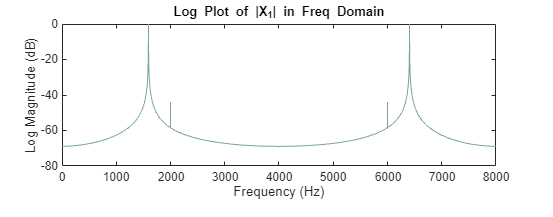
\includegraphics[width=0.5\linewidth]{figures/X1.png}
    \caption{Signal $x_1$ Frequency Spectrum}
    \label{fig:X1}
\end{figure}

In Figure \ref{fig:x1} and Figure \ref{fig:x1_zoom}, the signal can be seen in the time domain.  The signal looks as expected for two sinusoids being present, although the effect of Tone 2 is minimal.

\begin{figure}[H]
    \centering
    \includegraphics[width=0.5\linewidth]{figures/x1.png}
    \caption{Signal $x_1$ by Time}
    \label{fig:x1}
\end{figure}

\begin{figure}[H]
    \centering
    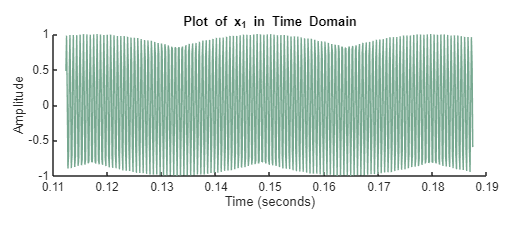
\includegraphics[width=0.5\linewidth]{figures/x1_zoom.png}
    \caption{Signal $x_1$ by Time}
    \label{fig:x1_zoom}
\end{figure}

Before any filtering is done, we can calculate the period of the dominant sinusoid.  From the frequency spectrum, we see that
\begin{align*}
    T = \frac{1}{1593 \unit{Hz}} = 620 \unit{$\micro$s},
\end{align*}
and from the plot in Figure \ref{fig:x1_timeT},
\begin{align*}
    T = 0.147625 \unit{s} - 0.147 \unit{s} = 625 \unit{$\micro$s}.
\end{align*}

\begin{figure}
    \centering
    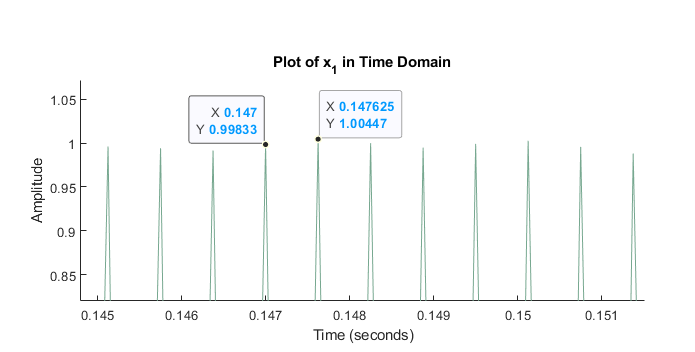
\includegraphics[width=0.5\linewidth]{figures/x1_timeperiod.png}
    \caption{Signal $x_1$ by Time with few Cycles}
    \label{fig:x1_timeT}
\end{figure}

The processing goal for Signal $x_1$ was to attenuate the tone of higher magnitude (Tone 1) so that the magnitude of Tone 1 was more than $30 \unit{dB}$ less than the magnitude of the tone of lower magnitude (Tone 2).  

A highpass filter was chosen for the first method, as that was the simplest option.  Because preserving linear phase is not important, IIR was chosen.  Additionally, the elliptic method was chosen as it yields the best magnitude response for a given order.  After several iterations, Filter 1 with the parameters in Table \ref{tab:x1_v2} was designed.

\begin{table}[H]
    \centering
    \begin{tabular}{c|cccc}
         Order & Fstop & Fpass & Astop & Apass \\ \hline
         7 & $1600  \unit{Hz}$ & $2000  \unit{Hz}$ & $73  \unit{dB} $ & $1  \unit{dB}$
    \end{tabular}
    \caption{Parameters for Filter 1 for Signal $x_1$}
    \label{tab:x1_v2}
\end{table}

Applying this filter to the signal yielded the response in Figure \ref{fig:X1_v2}.  The horizontal dark green line marks $-30\unit{dB}$, with the peak of Tone 2 at $0 \unit{dB}$.  Because the magnitude of Tone 1 is more than $30 \unit{dB}$ less than the magnitude of Tone 2, Filter 1 meets the specifications at order 7.  The signal's response can be heard with the \code{x1\_filtered7.wav} file in the \href{https://github.com/dbcometto/ece434_cpx2}{GitHub repository}.

\begin{figure}[H]
    \centering
    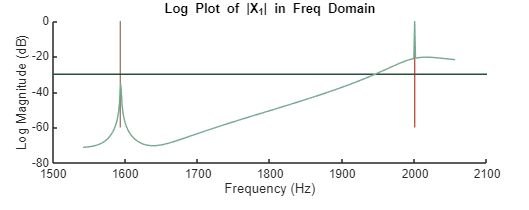
\includegraphics[width=0.5\linewidth]{figures/X1_filterv2.png}
    \caption{Response of Signal $x_1$ to Filter 1, Order 7}
    \label{fig:X1_v2}
\end{figure}

In order to reduce the order, a notching filter's poles and zeros were modified.  An order 2 filter, with a zero on Tone 1's frequency, was unable to reduce the magnitude enough.  Thus, Filter 2, an order 4 filter with the pole zero plot in Figure \ref{fig:x1_v10_polezero} was developed.

\begin{figure}[H]
    \centering
    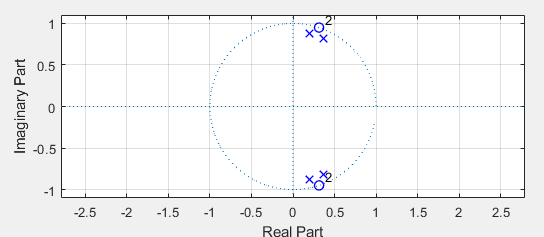
\includegraphics[width=0.5\linewidth]{figures/x1_v10_polezero.png}
    \caption{Pole Zero Plot of Filter 2 for Signal $x_1$}
    \label{fig:x1_v10_polezero}
\end{figure}

The locations of the poles and zeros are recorded in Table \ref{tab:x1_v10}.

\begin{table}[H]
    \centering
    \begin{tabular}{c|cccc}
         Order & & Zeros & Pole & Pole \\ \hline
         4 & Angle & $\pm 1.2519 \unit{rad}$  & $\pm 1.1519 \unit{rad}$ & $\pm 1.3519 \unit{rad}$ \\
         & Magnitude & $1$ & $0.9$ & $0.9$
    \end{tabular}
    \caption{Parameters for Filter 2 for Signal $x_1$}
    \label{tab:x1_v10}
\end{table}

The signal response of Filter 2 can be seen in Figure \ref{fig:X1_v10}.  The signal response can be heard in the \code{x1\_filtered4.wav} file in the \href{https://github.com/dbcometto/ece434_cpx2}{GitHub repository}.

\begin{figure}[H]
    \centering
    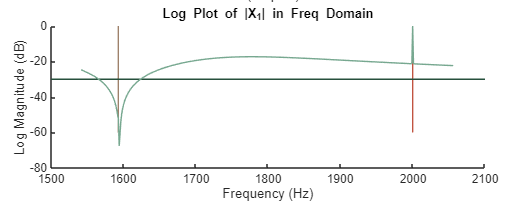
\includegraphics[width=0.5\linewidth]{figures/X1_filterv10.png}
    \caption{Response of Signal $x_1$ to Filter 2, Order 4}
    \label{fig:X1_v10}
\end{figure}

Because of the sharpness of the notching filter, the response looks different than expected for two tones.  Additionally, the sound is not identical to the first response.  Despite these factors, the majority of Tone 1's magnitude is below the $-30 \unit{dB}$ line, and thus Filter 2 meets the specifications with order 4.

The response of an order 2 notching filter can be seen in Figure \ref{fig:X1_v11}.  The filter is not able to bring Tone 1's magnitude below the $-30\unit{dB}$ specification.

\begin{figure}[H]
    \centering
    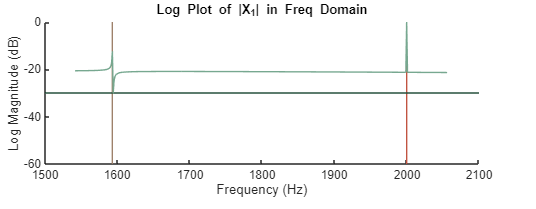
\includegraphics[width=0.5\linewidth]{figures/X1_filterv11.png}
    \caption{Response of Signal $x_1$ to an Order 2 Notching Filter}
    \label{fig:X1_v11}
\end{figure}

After filtering, we can again calculate the period of the dominant sinusoid.  From the frequency spectrum, we see that
\begin{align*}
    T = \frac{1}{2000 \unit{Hz}} = 500 \unit{$\micro$s},
\end{align*}
and from the plot in Figure \ref{fig:x1_timeT2},
\begin{align*}
    T = 0.207125 \unit{s} - 0.206625 \unit{s} = 500 \unit{$\micro$s}.
\end{align*}

\begin{figure}
    \centering
    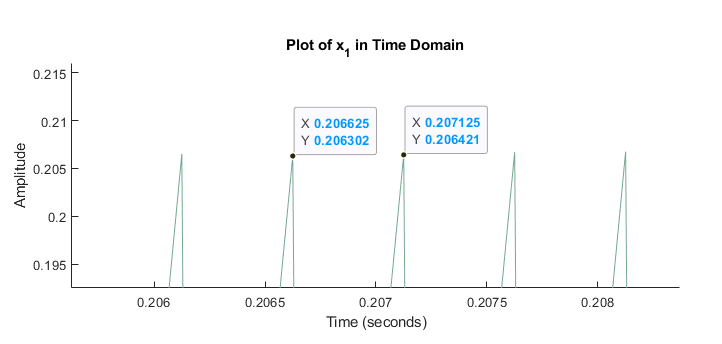
\includegraphics[width=0.5\linewidth]{figures/x1_timeperiod2.png}
    \caption{Signal $x_1$ After Filtering by Time with few Cycles}
    \label{fig:x1_timeT2}
\end{figure} 
\newpage
% !TEX root =./main.tex

\section{Signal $x_8$}

Signal $x_8$ contains an audio signal.  For most of the signal's duration, as can be seen in Figure \ref{fig:x8}, the audio is undisturbed.  However, at about the 8 second mark, narrowband jamming with 3 tones (plus a "tone" at DC) begins.  The tones can be clearly seen in the signal's frequency spectrum in Figure \ref{fig:X8}.  The unfiltered audio can be found in the \code{x8\_unfiltered.wav} file in the \href{https://github.com/dbcometto/ece434_cpx2}{GitHub repository}.

\begin{figure}[H]
    \centering
    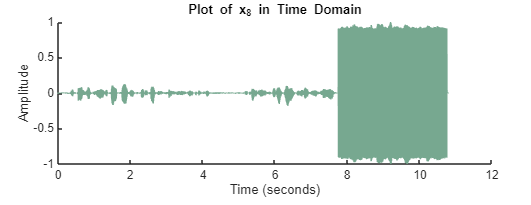
\includegraphics[width=0.5\linewidth]{figures/x8_prefilter.png}
    \caption{Signal $x_8$ over Time}
    \label{fig:x8}
\end{figure}

\begin{figure}[H]
    \centering
    \includegraphics[width=0.5\linewidth]{figures/X8_prefilter.png}
    \caption{Frequency Spectrum of Signal $x_8$}
    \label{fig:X8}
\end{figure}

Focusing on the portion of the frequency spectrum including the tones, it can be seen that the tones are at approximately $1573 \unit{Hz}$, $3151 \unit{Hz}$, and at $4726 \unit{Hz}$ (and at DC).
\begin{figure}[H]
    \centering
    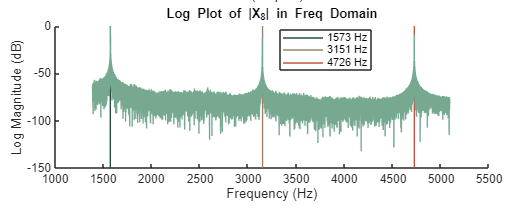
\includegraphics[width=0.5\linewidth]{figures/X8_prefilter_zoom.png}
    \caption{Frequency Spectrum of Signal $x_8$ near Interfering Tones}
    \label{fig:enter-label}
\end{figure}

Up to the 8 second mark, we are able to hear the message, ``He has been eight years upon a project for extracting sunbeams out of cucumbers... He told me, he did not doubt, that, in eight years more---."  The rest of the message (perhaps the secrets for extracting sunbeams from cucumbers?) has been jammed.  In order to recover the message, we must remove the interfering tones.

Again, a notching filter is indicated, as specific frequencies must be stopped.  This notching filter was built by placing poles and zeros.  Because we do not need to preserve linear phase, we can use poles (and thus create an IIR filter).  Converting the tone frequencies to normalized angular frequencies gave the locations of the zeros.  The poles were offset slightly in both angle and magnitude to maximize the notching effect while minimizing the effect on the surrounding frequencies.  For Filter 1, six zeros were used, one for each tone.  The pole zero plot can be seen in Figure \ref{fig:x8_v7_polezero}.

\begin{figure}[H]
    \centering
    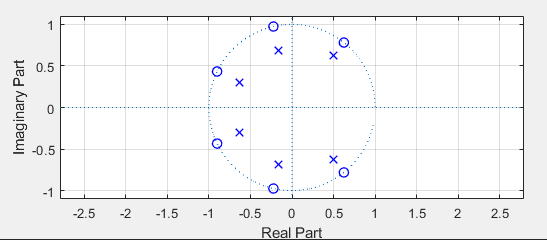
\includegraphics[width=0.5\linewidth]{figures/x8_v7_polezero.png}
    \caption{Pole Zero Plot of Filter 1 for Signal $x_8$}
    \label{fig:x8_v7_polezero}
\end{figure}

The locations of the poles and zeros are compiled in Table \ref{tab:x8_v7}.

\begin{table}[H]
    \centering
    \begin{tabular}{c|cccc}
         Order &      & Zero/Pole & Zero/Pole & Zero/Pole \\ \hline
         6 & Angle    & $\pm 0.8969 \unit{rad}$ & $\pm 1.7962 \unit{rad}$ & $\pm 2.6931 \unit{rad}$ \\
         & Magnitude  & $1$/$0.8$ & $1$/$0.8$ & $1$/$0.8$ 
    \end{tabular}
    \caption{Parameters for Filter 1 for Signal $x_8$}
    \label{tab:x8_v7}
\end{table}


Applying this filter to the signal results in the removal of the majority of the interference.  However, the tones are still present, albeit at a diminished volume.  The signal response can be seen in Figure \ref{fig:x8_v7_response}.  The audio information is clearly able to be heard, as can be verified in the \code{x8\_filter7.wav} file in the \href{https://github.com/dbcometto/ece434_cpx2}{GitHub repository}.
\begin{figure}[H]
    \centering
    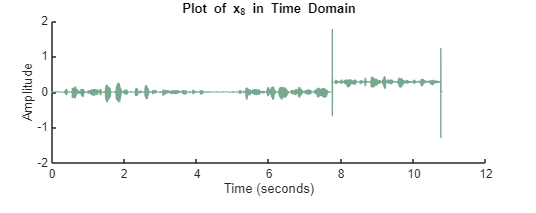
\includegraphics[width=0.5\linewidth]{figures/x8_filterv7.png}
    \includegraphics[width=0.5\linewidth]{figures/X8_filterv7.png}
    \caption{Response of Signal $x_8$ to Filter 1, Order 6}
    \label{fig:x8_v7_response}
\end{figure}

To fully remove the tones, the filter can be modified to order 12, placing two zeros at each tone's frequency.  This change results in Filter 2.  The pole zero plot for Filter 2 can be seen in Figure \ref{fig:x8_v5_polezero}.

\begin{figure}[H]
    \centering
    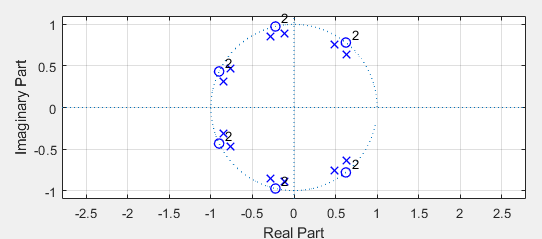
\includegraphics[width=0.5\linewidth]{figures/x8_v5_polezero.png}
    \caption{Pole Zero Plot of Filter 2 for Signal $x_8$}
    \label{fig:x8_v5_polezero}
\end{figure}

The locations of the zeros are the same as in Filter 1.  The poles' magnitude were increased to $0.9$, and they are placed $\pm 0.1 \unit{rad}$ from the angle of their corresponding zero.

The signal response to Filter 2 can be seen in Figure \ref{fig:x8_v5_response}.  Now, the tones have been completely removed, but there is a DC shift and two pops can be heard during the jammed portion of the signal.  The output audio can be heard in the \code{x8\_filter12.wav} file in the \href{https://github.com/dbcometto/ece434_cpx2}{GitHub repository}.  It is not necessary to remove these artifacts, as they do not interfere with the content of the signal.

\begin{figure}[H]
    \centering
    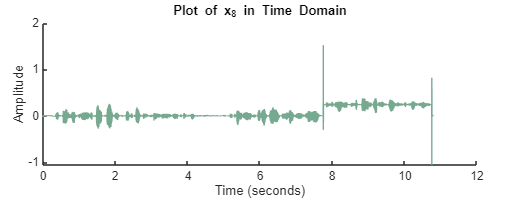
\includegraphics[width=0.5\linewidth]{figures/x8_filterv5.png}
    \includegraphics[width=0.5\linewidth]{figures/X8_filterv5.png}
    \caption{Response of Signal $x_8$ to Filter 2, order 12}
    \label{fig:x8_v5_response}
\end{figure}

However, in order to maximally enhance the audio and remove these final artifacts, zeros and corresponding poles are added near DC, resulting in Filter 3.  The response to Filter 3 can be seen in Figure \ref{fig:x8_14}

\begin{figure}[H]
    \centering
    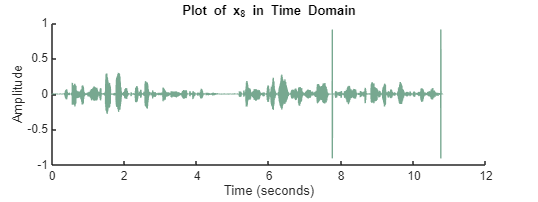
\includegraphics[width=0.5\linewidth]{figures/x8_filter11.png}
    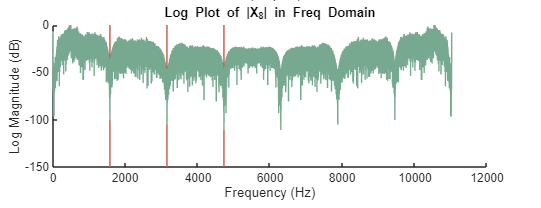
\includegraphics[width=0.5\linewidth]{figures/X8_filterv11.png}
    \caption{Response of Signal $x_8$ to Filter 3}
    \label{fig:x8_14}
\end{figure}

Additionally, the pops are manually removed from the audio by setting the corresponding portions of the time signal to zero.  A final, completely clean output can be seen in Figure \ref{fig:x8_clean}, and heard in the \code{x8\_filterNoPop.wav} file in the \href{https://github.com/dbcometto/ece434_cpx2}{GitHub repository}.

\begin{figure}[H]
    \centering
    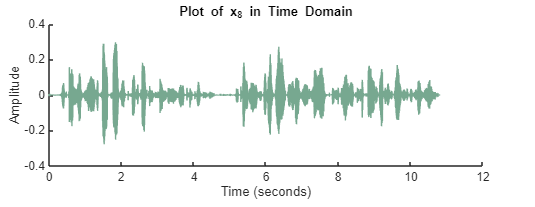
\includegraphics[width=0.5\linewidth]{figures/x8_nopops.png}
    \caption{Signal $x_8$ after Filter 3 and Editing}
    \label{fig:x8_clean}
\end{figure}

As can be heard following the application of any of the 3 filters, the complete message is, ``He has been eight years upon a project for extracting sunbeams out of cucumbers... He told me, he did not doubt, that, in eight years more, he should be able to supply the governor’s gardens with sunshine."  Originally, I misheard several of the words.  However, a Google search revealed that it is an abridged quote from \textit{Gulliver's Travels}, which enabled me to correct the words that I heard incorrectly. 
\newpage
% !TEX root =./main.tex

\section{Signal}
 
\newpage
% !TEX root =./main.tex

\section{Signal $x_4$}

Signal $x_4$ is an audio signal.  However, it has been jammed with a wideband jammer, producing the data seen in Figure \ref{fig:x4}.  This is clearly unintelligible, and the unfiltered audio can be found in the \code{x4\_unfiltered.wav} file in the \href{https://github.com/dbcometto/ece434_cpx2}{GitHub repository}.

\begin{figure}[H]
    \centering
    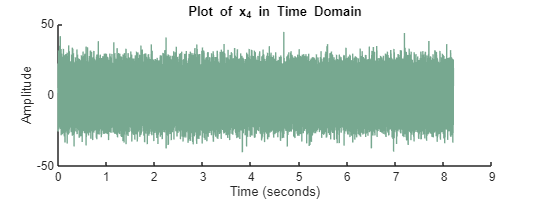
\includegraphics[width=0.5\linewidth]{figures/x4.png}
    \caption{Signal $x_4$ over Time}
    \label{fig:x4}
\end{figure}

The frequency spectrum in Figure \ref{fig:X4} similarly shows that a large amount of noise has been added to the signal.  

\begin{figure}[H]
    \centering
    \includegraphics[width=0.5\linewidth]{figures/X4.png}
    \caption{Frequency Spectrum of Signal $x_4$}
    \label{fig:X4}
\end{figure}


However, notice that the noise appears to begin just before $1000 \unit{Hz}$, as can be seen in Figure \ref{fig:X4_1000}.  This will enable us to extract the majority of the information in the original audio signal, as a large portion of the speech range of frequencies has been preserved.


\begin{figure}[H]
    \centering
    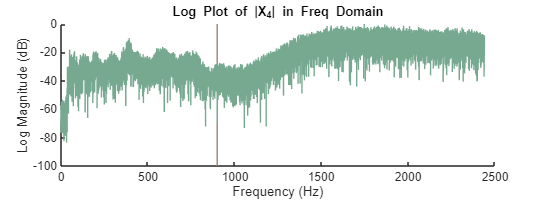
\includegraphics[width=0.5\linewidth]{figures/X4_1000.png}
    \caption{Frequency Spectrum of Signal $x_4$, focused on Audible Frequencies}
    \label{fig:X4_1000}
\end{figure}

In order to filter out the noise that is overpowering the audio, we will use a low pass filter.  Also, because preserving linear phase is important, we will use an FIR filter.  First, we will try to decipher the message, allowing our order to be higher.  After several iterations, we arrive at the design for Filter 1.  The parameters for Filter 1 can be seen in Table \ref{tab:x4_v22}.  The equiripple method yields the best magnitude response for a given order.

\begin{table}[H]
    \centering
    \begin{tabular}{c|cccc}
         Order & Fpass & Fstop & Apass & Astop \\ \hline
         56 & $800  \unit{Hz}$ & $2000  \unit{Hz}$ & $1  \unit{dB} $ & $100  \unit{dB}$
    \end{tabular}
    \caption{Parameters for Filter 1 for Signal $x_4$}
    \label{tab:x4_v22}
\end{table}

Applying the filter to the signal yields the following time and frequency responses in Figure \ref{fig:x4_v22_both}.


\begin{figure}
    \centering
    \includegraphics[width=0.5\linewidth]{figures/x4_v22.png}
    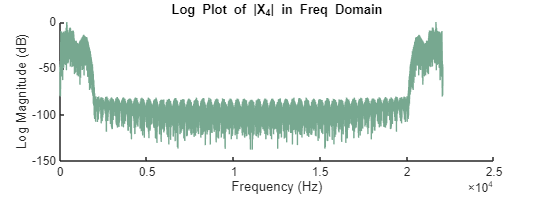
\includegraphics[width=0.5\linewidth]{figures/X4_v22.png}
    \caption{Response of Signal $x_4$ to Filter 1, Order 56}
    \label{fig:x4_v22_both}
\end{figure}

This removes all of the noise, but also removes portions of the speech information.  Despite this, we are still able to interpret the information.  At first, I was only able to hear, ``huh, what is that the light... crush your enemies... it is given before you... and walalalalalanight." Putting this into a google search brought me to a Reddit page quoting Conan the Barbarian.  I followed this lead, and came across a YouTube video that contains the full quote, ``Conan, what is best in life? To crush your enemies, see them driven before you, and to hear the lamentations of their women."  While still distorted, it is easy to hear the words once they are known.  This audio can be heard in the \code{x4\_goodAudio.wav} file in the \href{https://github.com/dbcometto/ece434_cpx2}{GitHub repository}.

Pushing this idea to its maximum, progressively adjusting the parameters enabled lowering the order of the filter to order 5.  The specifications for Filter 2 can be seen in Table \ref{tab:x4_v21}. 

\begin{table}[H]
    \centering
    \begin{tabular}{c|cccc}
         Order & Fpass & Fstop & Apass & Astop \\ \hline
         5 & $100  \unit{Hz}$ & $3300  \unit{Hz}$ & $4  \unit{dB} $ & $39  \unit{dB}$
    \end{tabular}
    \caption{Parameters for Filter 2 for Signal $x_4$}
    \label{tab:x4_v21}
\end{table}

Applying Filter 2 to the signal yields the time and frequency response in Figure \ref{fig:x4_v21_both}.

\begin{figure}[H]
    \centering
    \includegraphics[width=0.5\linewidth]{figures/x4_v21.png}
    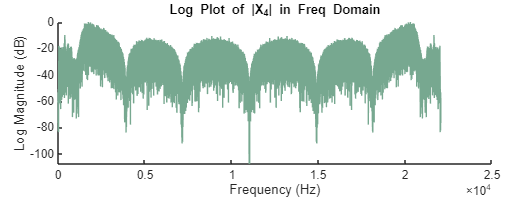
\includegraphics[width=0.5\linewidth]{figures/X4_v21.png}
    \caption{Response of Signal $x_4$ to Filter 2, Order 5}
    \label{fig:x4_v21_both}
\end{figure}

This yields quiet audio with a lot of hissing noise on top.  However, it is still easy to make out the words.  In many ways, the audio sounds better: it had less of the audio information removed.  The audio is just less uncovered.  This response can be heard in the \code{x4\_barelyAudible.wav} file in the \href{https://github.com/dbcometto/ece434_cpx2}{GitHub repository}.


 
\newpage
% !TEX root =./main.tex

\section{Signal}  
\newpage
% !TEX root =./main.tex

\section{Conclusion}

For each of the five signals provided for Computer Exercise 2 (CPX 2), the processing goal was met with a filter of minimum order.  In summary, in Signal $x_1$, the louder tone was attenuated so that the quieter tone was more than $30 \unit{dB}$ greater in magnitude.  In Signal $x_8$, the secrets of extracting sunshine from cucumbers was revelaed after an attempted jamming.  In Signal $x_3$, interference from a power line in an electrocardiogram (ECG) was removed.  In Signal $x_4$, the secret to a good life according to Conan the Barbarian was revealed after another attempted jamming.  In Signal $x_7$, ten test tones were modified to be within $1 \unit{dB}$ of a specified magnitude.

For the filters for Signals $x_1$ and $x_8$, preserving linear phase was not important, and thus infinite impulse response (IIR) filters were used because they have a better magnitude response for a given order.  For Signals $x_3$ and $x_4$, preserving linear phase was important, and thus finite impulse response (FIR) filters were used.  For details on each filter, see the signal's respective section.  

Throughout this experience, I gained experience working with digital filters, in both design and application.  Additionally, I built upon my "signal hunting" skills that had been built in CPX 1 in order to understand the content of the signals, a necessary prerequisite to processing them appropriately.  I also gained more experience with audio processing in Matlab, and learned how to export to \code{.wav} files.  Additionally, I gained more experience in \LaTeX, which is always helpful.

For access to the Matlab \code{.mlx} files, source signal data, filter designer session \code{.fda} file, filter taps \code{.bin} files, and output \code{.wav} sound files, see the project's GitHub repository at \url{https://github.com/dbcometto/ece434_cpx2}.




\section*{Documentation}

I did all my own work.  I had various conversations with classmates, including C1C Csicsila and C1C Chen.  However, no changes were made based on those conversations.  Additionally, I used Google (\url{https://brainly.com/question/2233369}) to find the cucumber quote and YouTube (\url{https://www.youtube.com/watch?v=V30tyaXv6EI}) to find the Conan the Barbarian quote.  I used various resources, including overleaf.com, for Latex help.  I also used various ECG interpretation resources, including \href{https://clinical.stjohnwa.com.au/medical-library/ecg-library/introduction-overview/introduction-to-the-ecg#:~:text=Generated\%20when\%20there\%20is\%20movement,direction\%20of\%20these\%20electrical\%20impulses.&text=From\%20Atrial\%20depolarisation\%20(start\%20in,from\%20right\%20to\%20left\%20atrium.}{this article}, several YouTube videos, and several Google images of atrial fibrillation.  I also used the Mathworks website for Matlab help, for various syntax issues, and additionally for the \code{upsample} function, in an attempt to play the ECG data (until I learned that real ECGs use sonification to play the data, which makes way more sense).  I also used my notes from Math 342 Numerical Analysis and the Remez algorithm Wikipedia page.  Additionally, C1C Csicsila asked me a question regarding why it is worth finding the period in both the time domain and frequency domain, and that led me to realize I had forgot to answer several questions. 




% Endnotes - activate if needed
%%% in the text, you can use /endnote{} 
%%% command to insert endnotes

%\newpage
%\theendnotes 
%\newpage



% Bibliography 
%\printbibliography

\end{document}
